\documentclass[mcp]{article}
%\documentclass[11pt, twocolumn]{article}

\usepackage[colorinlistoftodos]{todonotes}
\usepackage{graphicx}
\graphicspath{ {./images/} }

%\usepackage{fullpage}
\usepackage[margin=1in,headheight=13.6pt]{geometry}
\usepackage{amsfonts,amsthm}
\usepackage{amsmath}
%\numberwithin{figure}{section} % numbering in each subsection
\numberwithin{table}{section}
\usepackage{setspace}
\usepackage{url}
\usepackage{lscape} %% rotating table
\usepackage{rotating}
\usepackage{authblk}
\usepackage{subcaption}
\usepackage{hyperref}
\usepackage{xcolor} %\[table,dvipsnames]
%\usepackage{makecell}
%\usepackage{array}

% remove number of section in the title
\makeatletter
\def\@seccntformat#1{%
  \expandafter\ifx\csname c@#1\endcsname\c@section\else
  \csname the#1\endcsname\quad
  \fi}
\makeatother

\usepackage{caption}

%% to remove zero preceding section number.
\renewcommand\thesection{\arabic{section}}
\renewcommand\thesubsection{\thesection.\arabic{subsection}}

\usepackage{tabulary,multirow,multicol,rotating}
\usepackage[backend=biber, citestyle=numeric, bibstyle=authoryear, sorting=none]{biblatex}
\addbibresource{bibliography.bib}

\makeatletter
\input{numeric.bbx}
\makeatother

\definecolor{Red}{rgb}{0.60,0.00,0.00}
\definecolor{Blue}{rgb}{0.00,0.00,0.75}
\definecolor{LightYellow}{rgb}{1.00,0.97,0.68}
\definecolor{Green}{rgb}{0.30, 0.60, 0.30}
\definecolor{MyLightMagenta}{cmyk}{0.1,0.8,0,0.1} 
\definecolor{cornflowerblue}{rgb}{0.39, 0.58, 0.92}
\definecolor{darkorange}{rgb}{0.8, 0.4, 0}
\definecolor{LightPurple}{rgb}{1, 0.51, 0.98}
\definecolor{DarkPurple}{rgb}{0.54, 0.27, 0.53}
\definecolor{Purple1}{rgb}{0.83, 0.29, 0.95}
\definecolor{Purple2}{rgb}{0.97, 0.12, 0.59}
\definecolor{change}{rgb}{0.39, 0.58, 0.92}

\definecolor{function}{RGB}{0, 112, 192}
\definecolor{group}{rgb}{0.39, 0.58, 0.92}
\definecolor{ratio}{rgb}{1, 0.6, 0.16}
\definecolor{feature}{rgb}{0.83, 0.32, 0.48}
\definecolor{subject}{rgb}{0.6, 0.3, 0.09}
\definecolor{run}{rgb}{0, 0.68, 0.17}

\usepackage{array}
\newcolumntype{C}[1]{>{\centering\let\newline\\\arraybackslash\hspace{0pt}}m{#1}}
\setlength{\tabcolsep}{2pt}

%% for comments
\newcommand{\ignore}[1]{}
\def\todo#1{{\color{red}[#1]}}
\def\change#1{{\color{cornflowerblue}#1}}
\newenvironment{todolong}{\color{red}[TODO:}{]}
\def\ov#1{{\color{red}#1}}
\def\note#1{{\color{OliveGreen}[NOTE: #1]}}
\def\added#1{{\color{blue}[ADDED: #1]}}
\def\devon#1{{\color{green}[4Devon: #1]}}

\def\eqref#1{Eq.~(\ref{eq:#1})}
\def\figshortref#1{{\bf Fig.~\ref{fig:#1}}}
\def\figref#1{{\bf Figure~\ref{fig:#1}}}
\def\secref#1{{\bf Section~\ref{sec:#1}}}
\def\tabref#1{{\bf Table~\ref{tab:#1}}}

\usepackage{xr}
\externaldocument[supp-]{../supplementary/ptm_sm}
%\def\sfigref#1{{\bf Supplementary Fig.~\ref{fig:#1}}}
%\def\snoteref#1{{\bf Supplementary Note~\ref{sec:#1}}}
%\def\snoteshortref#1{{\bf Suppl. Note~\ref{sec:#1}}}
%\def\stabref#1{{\bf Supplementary Table~\ref{tab:#1}}}

%%% should be change =2
\linespread{1}

\usepackage{fancyhdr}
\pagestyle{fancy}
\fancyhead[L]{MSstatsPTM: Statistical relative quantification of PTMs}

%\date{\vspace{-5ex}} % to remove date in the title

\renewcommand{\deg}{\ensuremath{^{\circ}}\xspace}
\newcommand{\dd}[1]{\mathrm{d}#1}

%%%%%%%%%%%%%%%%%%%%%%%%%%%%%%%%%%%%%%%%%%%%%%%%%%%%%%%%%%%%%%%%%%%%%%%
%%%%%%%%%%%%%%%%%%%%%%%%%%%%%%%%%%%%%%%%%%%%%%%%%%%%%%%%%%%%%%%%%%%%%%%
%%%%%%%%%%%%%%%%%%%%%%%%%%%%%%%%%%%%%%%%%%%%%%%%%%%%%%%%%%%%%%%%%%%%%%%

\title{MSstatsPTM: Statistical relative quantification of post-translational modifications in bottom-up mass spectrometry-based proteomics}

\author[1]{Devon~Kohler}
\author[2]{Tsung-Heng~Tsai}
\author[4]{Erik~Verschueren}
\author[1]{Ting~Huang}
\author[3]{Trent~Hinkle}
\author[3]{Lilian~Phu}
\author[3]{Meena~Choi*}
\author[1]{Olga~Vitek*}
\affil[1]{Khoury College of Computer Science, Northeastern University, Boston, MA, USA}
\affil[2]{Kent State University, Kent, OH, USA}
\affil[3]{MPL, Genentech, South San Francisco, CA, USA}
\affil[4]{ULUA BV, Arendstraat 29, 2018 Antwerp, Belgium}
\affil[*]{Corresponding Authors}
%\affil[]{MSstatsPTM: Statistical relative quantification of PTMs}

\date{}

\begin{document}

\maketitle


%%%%%%%%%%%%%%%%%%%%%%%%%%%%%%%%%%%%%%%%%%%%%%%%%%%%%%%%%%%%%%%%%%%%%%%
%%%%%%%%%%%%%%%%%%%%%%%%%%%%%%%%%%%%%%%%%%%%%%%%%%%%%%%%%%%%%%%%%%%%%%%
\begin{abstract}

Liquid chromatography coupled with bottom up mass spectrometry (LC-MS/MS)-based proteomics is increasingly used to detect changes in post-translational modifications (PTMs) in samples conditions. Analysis of data from such experiments faces numerous statistical challenges. These include the low abundance of modified proteoforms, the small number of observed peptides that span modification sites, and confounding between changes in the abundance of PTM and the overall changes in the protein abundance. Therefore, statistical approaches for detecting differential PTM abundance must integrate all the available information pertaining to a PTM site, and consider all the relevant sources of confounding and variation. In this manuscript we propose such a statistical framework, which is versatile, accurate, and leads to reproducible results. The framework requires an experimental design, which quantifies, for each sample, both peptides with post-translational modifications and peptides from the same proteins with no modification sites. The proposed framework supports both label-free and tandem mass tag (TMT)-based LC-MS/MS acquisitions. The statistical methodology separately summarizes the abundances of peptides with and without the modification sites, by fitting separate linear mixed effects models appropriate for the experimental design. Next, model-based inferences regarding the PTM and the protein-level abundances are combined to account for the confounding between these two sources. Evaluations on computer simulations, a spike-in experiment with known ground truth, and three biological experiments with different organisms, modification types and data acquisition types demonstrate the improved fold change estimation and detection of differential PTM abundance, as compared to currently used approaches. The proposed framework is implemented in the free and open-source R/Bioconductor package $MSstatsPTM$. 

\end{abstract}

%%%%%%%%%%%%%%%%%%%%%%%%%%%%%%%%%%%%%%%%%%%%%%%%%%%%%%%%%%%%%%%%%%%%%%%
%%%%%%%%%%%%%%%%%%%%%%%%%%%%%%%%%%%%%%%%%%%%%%%%%%%%%%%%%%%%%%%%%%%%%%%
\clearpage
\section{Introduction}

Signaling mechanisms allow cells to mount a fast and dynamic response to a multitude of biomolecular events. Signaling is facilitated by the modification of proteins at specific residues, acting as molecular on/off switches~\cite{Deribe,Cohen,Bludau2022}. Characterizing relative abundance of a modification site's occupancy repertoire across experimental conditions provides important insights~\cite{Mann}. For example, meaningful patterns of changes in post-translational modifications (PTMs) abundance can serve as biomarkers of a disease~\cite{Petushkova_2017}. Alternatively, distinguishing the quantitative changes in a PTM from the overall changes of the protein abundance helps gain insight into biological and physiological processes operating on a very short timescale~\cite{Chandramouli:2009}\cite{Kim2016}. This helps to distinguish between relative site occupancy changes at steady-state protein levels, typical for short time-scale signaling events, and observed relative changes of PTMs as a result of underlying gene expression or protein abundance levels.

Bottom-up liquid chromatography coupled with tandem mass spectrometry (LC-MS/MS) is a tool of choice for unbiased and large-scale identification and quantification of proteins and their PTMs~\cite{Kall:2011ub,Roepstorff}. However, LC-MS-based interrogation of the modified proteome is challenging, for a number of reasons. First, the relatively lower abundance of modified proteoforms dictates that a global interrogation can only be achieved through large-scale enrichment protocols with modification-specific antibodies or beads \cite{Huang:2014}. Variability in the enrichment efficiency inevitably affects the reproducibility of the number of spectral features (e.g., peptide precursor ions or their fragments) and their intensities. Second, contrary to the often large number of identified peptides that can be used to quantify protein abundance, there are relatively few representative peptides that span a modification site, and there may be multiple modified sites on a single peptide~\cite{Mann}. Third, unless early signaling events are interrogated, the interpretation of the relative changes in modification occupancy are inherently confounded with changes in the overall protein abundance, complicating the interpretation of the results \cite{Olsen:2013}. Finally, technological aspects of bottom-up MS experiments, such as presence of labeling by tandem mass tag (TMT), introduce additional sources of uncertainty and variation.

The technological difficulties in PTM identification and quantification increase the uncertainty and the variation in the data, and challenge the downstream statistical analyses. Frequently data from these experiments are analyzed using statistical methods that were not originally designed for this task. Researchers use methods such as $t$-test\cite{Kalpic:2011}, Analysis of Variance\cite{girden:1992}, or Limma\cite{Ritchie_15a}, by taking as input the intensity ratios of modified and unmodified peptide features, and comparing the mean abundance of different PTM sites. Such approaches do not fully account for all the sources of uncertainty. As the result, these approaches are either not directly applicable to experiments with non-trivial designs (such as experiments with multiple conditions, paired and time course designs, and experiments with labeling), or require the analysts to exercise non-trivial statistical expertise.

This manuscript proposes a versatile statistical analysis framework that accurately detects relative changes in post-translational modifications. The framework requires an experimental design, which quantifies, for each sample, both the peptides with post-translational modifications, and peptides from the same proteins with no modification sites. The framework supports data-dependent acquisitions (DDA) that are label-free or tandem mass tag (TMT)-based. The statistical methodology separately summarizes the abundances of peptides with and without the modification sites, and fits separate linear mixed effects models that reflect the biological and technological aspects of the experimental design. Next, model-based inferences regarding the PTM and the protein-level abundances are combined to account for the confounding between these two sources.

We evaluated the proposed framework on two datasets from computer simulations, one benchmark controlled mixture, and three biological investigations. The datasets illustrate a diverse set of organisms, modification types, acquisition methods and experimental designs, showing the applicability of the framework to a variety of situations. By appropriately leveraging the information from the unmodified peptides, the proposed approach improved the accuracy of the estimates of PTM fold changes and produced a better calibrated false positive rate of detecting differentially abundant PTMs as compared to existing methods. In particular, accounting for the confounding from protein abundance allowed us to characterize the true effect of the modification, avoiding the need for more manual and time intensive follow-up investigation.

The proposed approach is implemented as a freely available open source R package $MSstatsPTM$, as part of the $MSstats$ family of packages \cite{Choi:2014,Huang:2020}, and is available on Bioconductor.

\section{Experimental procedures}

\subsection*{Data overview and availability}

Table \ref{tab:dataDescription} summarizes the experiments. Two computer simulations had known ground truth, and varied in experimental realism. The first simulation produced a perfectly clean dataset, with many replicates and no missing values. The second simulation introduced real-world characteristics, such as limited modified features and missing values. Details of computer simulations are available on GitHub (\url{https://github.com/devonjkohler/MSstatsPTM_simulations}).

One spike-in experiment also had known changes in modified spike-in peptides, but had real-world experimental characteristics. Finally, three biological experiments demonstrated the applicability of the proposed approach across different biological organisms, modifications, experimental designs and acquisition strategies. Details of the experimental data, R scripts with $MSstatsPTM$ analysis, and results of the statistical analysis are available in MassIVE.quant (\url{https://massive.ucsd.edu/ProteoSAFe/static/massive-quant.jsp}) \cite{Choi:2020}. 

Additional details on every dataset are available in Supplementary Section 2.

\subsection*{Dataset 1: Computer simulation 1 - Label-free}
\label{sec:comp_sim_procedure1}

{\bf Simulation design:} The simulation represented an idealistic case. 24 synthetic label-free datasets were generated with different experimental designs and different biological variation. In each dataset, 1,000 proteins had 10 unmodified features per protein. Each of the 1,000 proteins had one PTM. Each PTM was represented by 10 modified features. The PTMs of 500 proteins had a differential fold change between conditions, while the other 500 proteins were generated with no changes in abundance between conditions. Furthermore, the fold changes of half of the 500 differential PTMs were fully masked by changes in the unmodified protein. Additionally, the fold change of half the 500 non-differential PTMs was entirely due to changes in the unmodified protein. All the differential PTMs were generated with an expected log fold change of 0.75 between conditions. 

Each simulation was generated with random biological variation. The observed peptide abundances were simulated by adding random noise $\mathcal{N}(0,\sigma^2)$ to the deterministic abundances described above. Two values $\sigma^2 = \{.2, .3\}$ were motivated by the experimental datasets in this manuscript.

\medskip \noindent {\bf Evaluation:} We evaluated the ability of the statistical methods to correctly detect which PTMs were simulated with changes between conditions and which were not. We evaluated the methods ability to avoid false positives (i.e. specificity), accurately estimate the fold change between conditions, and analyzed the sensitivity of detecting differentially abundant PTMs. Each method was used to analyze changes in PTM abundance in the presence of confounding with changes in the unmodified protein, and with this confounding removed.

\subsection*{Dataset 2: Computer simulation 2 - Label-free missing values and low features}
\label{sec:comp_sim_procedure2}

{\bf Simulation design:} The data were simulated as above, while providing a more realistic representation of the experiments. The feature counts and the proportion of missing values were as observed on average over all the the experimental datasets in this manuscript. Specifically, PTMs were simulated with 2 modified peptide features, and unmodified proteins were simulated with 10 features. Additionally, 20\% of observations for both modified and unmodified peptides were missing completely at random. 

\medskip \noindent {\bf Evaluation:} The methods were evaluated in the same way as above. We evaluated their ability to correctly detect PTM's specificity, fold change estimation, and sensitivity. These statistics were analyzed both in the presence of, and without, confounding with changes in the unmodified protein.
 
\subsection*{Dataset 3: SpikeIn benchmark - Ubiquitination - Label-free}
\label{sec:exp_proc_dataset3}

\medskip \noindent {\bf Experimental Design:} Figure \ref{fig:benchmark-design}(a) overviews the experimental design. Four mixtures (i.e., conditions) were created with varying amounts of human lysate, background {\it E. coli} lysate, and human spike-in ub-peptide mixture. Unmodified peptides from human lysate were viewed as the global proteome. Background {\it E. coli} lysate were used to equalize total protein levels prior to enrichment or global protein profiling between Mix 1 and 3, and between Mix 2 and 4.  50 heavy-labeled KGG motif peptides from 20 human proteins were used as spike-in peptides in a mixed background of lysates from {\it E. coli} and a human cell line. Quantitative changes in protein and site abundance of these 20 human proteins were the target of the benchmark. In particular, we distinguish the changes in the abundances of the modified peptides (i.e., unadjusted changes) and the changes of their abundance relative to the changes in the abundances of the human lysate (i.e., protein-level adjusted changed). The true log-fold changes between the relevant components of the relevant mixtures are summarized in Figure \ref{fig:benchmark-design}(b).  Two replicate mixtures were created per condition. 

\medskip \noindent {\bf Data acquisition:} Each mixture was analyzed with KGG enrichment, and without KGG enrichment (i.e., in a global profiling run), with label-free LC-MS/MS. There was a 90.2\% overlap of protein identifications between the identified background modified peptides and proteins that were quantified in the global profiling run.

\medskip \noindent {\bf Evaluation:} We expect the spike-in peptides to change corresponding to the values in Figure \ref{fig:benchmark-design}(b). These peptides are treated as positive controls in all comparisons except Mix 1 vs Mix 4. Additionally, the background {\it E. coli} lysate peptides are treated as negative controls and are not expected to change in any comparison. Therefor we evaluated the statistical methods ability to avoid false positives, as well as their sensitivity in detecting the differentially abundant spike-in peptides and accurately estimate their expected fold change.


\todo{Here is the place to describe: 'we expect XXX to not change'. Therefore we evaluated the ability of statistical methods to avoid false positives (i.e., specificity). We expect XXX to have fold changes XXX between conditions XXX. We evaluated the accuracy of estimation of fold changes... and the sensitivity of detecting differentially abundant...}  
%
\todo{I think some mixtures are not comparable because the total protein amount is not the same. I believe only in Mix 1 vs 2 and Mix 3 vs 4 are comparable. I do not think it is correct to compare Mix 1 vs 3 and 2 vs 4 directly because they differ in the total amount of the proteome. Or was it normalized based on what we know is the same? If yes, we need to describe in the beginning of 'Evaluation'}  \todo{The unadjusted proteins... estimation... The adjusted proteins... estimation... Positive controls... Negative controls...}

\subsection*{Dataset 4: Human - Ubiquitination - 1mix-TMT}
\label{sec:exp_proc_dataset4}

\medskip \noindent {\bf Experimental Design:}  Luchetti et al. \cite{LUCHETTI2021} profiled human epithelial cells engineered to express IpaH7.8 under a dox inducible promoter. Uninfected cells were measured at 0 and 6 hours, while cells infected with {\it Shigella flexneri} ({\it S. flexneri}) bacteria were measured at 1, 2, 4, and 6 hour increments, resulting in six total conditions. Shigella ubiquitin ligase IpaH7.8 was shown to function as an inhibitor of the protein gasdermin D (GSDMD). GSDMD was actively degraded when IpaH7.8 expression was induced by dox treatment in human cells.

\medskip \noindent {\bf Data acquisition:} 11 samples were allocated to 1 TMT mixture in an unbalanced group comparison design. All conditions were allocated two biological replicates except for the Dox1hr condition, which was allocated one replicate. The ubiquitinated peptides, and the total proteome (i.e., global profiling) were each conducted in a single LC-MS/MS run. There was a 95\% overlap between the identified modified peptides and proteins that were quantified in the global profiling run.

\medskip \noindent {\bf Evaluation:} We evaluated the ability of the statistical methods to detect changes in the abundance of modified peptides both before and after adjusting for changes in global protein abundance. The six condition were labeled Dox1hr, Dox2hr, Dox4hr, Dox6hr, NoDox0hr, and NoDox6hr. All conditions were compared with each other, resulting in 15 pairwise comparisons. Since the dataset was a biological investigation, the true positive modifications were unknown.


\subsection*{Dataset 5: Mouse - Phosphorylation - 2mix-TMT}
\label{sec:exp_proc_dataset5}


\medskip \noindent {\bf Experimental Design:} Maculins et al. \cite{Maculins} studied primary murine macrophages infected with {\it S. flexneri}. The experiment quantified the abundance of total protein and of phosphorylation in wild type (WT), and in ATG16L1-deficient (cKO) samples, uninfected and infected with {\it S. flexneri}. The abundance of total protein and post-translation modifications were quantified at three time points, uninfected, early infection (45-60 minutes), and late infection (3-3.5 hours). 

\medskip \noindent {\bf Data acquisition:} 22 biological samples were allocated to 2 TMT mixtures in an unbalanced design, with 11 samples allocated to each mixture. 16 replicates were spread equally between the early and late WT and cKO conditions, resulting in four replicates per condition. Both the uninfected WT and cKO contained 3 replicates, with mixture one allocating one replicate to uninfected WT and two replicates to uninfected cKO. Conversely, mixture two contained one replicate of uninfected cKO and two uninfected WT. This experiment included a total proteome (i.e., a global profiling run) and a phosphopeptide enrichment run. There was a 90\% overlap between the identified modified peptides and proteins that were quantified in the global profiling run.

\medskip \noindent {\bf Evaluation:} We evaluated the ability of the statistical methods to detect changes in the abundance of modified peptides both before and after adjusting for changes in global protein abundance. The six condition were labeled KO\_Uninfect, KO\_Early, KO\_Late, WT\_Uninfect, WT\_Early, and WT\_Late. 9 total comparisons were made, namely KO\_Early-WT\_Early, KO\_Late-WT\_Late, KO\_Uninfected-WT\_Uninfected, KO\_Early-KO\_Uninfected, KO\_Late-KO\_Uninfected, WT\_Early-WT\_Uninfected, WT\_Late-WT\_Uninfected, Infected-Uninfected, and KO-WT. Since the dataset was a biological investigation, the true positive modifications were unknown.


\subsection*{Dataset 6: Human - Ubiquitination - Label-free no global profiling run}
\label{sec:exp_proc_dataset6}

\medskip \noindent {\bf Experimental Design:} Cunningham et al. \cite{Cunningham2015} investigated the relationship between USP30 and protein kinase PINK1, and their association with Parkinson’s Disease. The experiment profiled ubiquitination sites, and analyzed changes in the modified site abundance. The experiment had four conditions, CCCP, USP30 over expression (USP30 OE), Combo, and Control. Cell lines were used to create two biological replicates per condition. The abundance of modified peptides was quantified with label-free LC-MS/MS.

\medskip \noindent {\bf Data acquisition:} This experiment did not include a separate global profiling run to measure unmodified peptides. In addition to low feature counts for unmodified peptides,  this lead to substantially fewer matches between modified and unmodified peptides. There was a 41.9\% overlap between the identified background modified peptides and proteins that were quantified in the global profiling run.

\medskip \noindent {\bf Evaluation:} We evaluated the ability of the statistical methods to detect  changes in the abundance of modified peptides both before and after adjusting for changes in global protein abundance. All the conditions were compared with each other in a full pairwise comparison, resulting in 6 comparisons. Since the dataset is a biological investigation, the true positive modifications were unknown.

%%%%%%%%%%%%%%%%%%%%%%%%%%%%%%%%%%%%%%%%%%%%%%%%%%%%%%%%%%%%%%%%%%%%%%%
\section*{Background}

\subsection*{Goals of PTM characterization, input to statistical analyses, and notation}

Consider a label-free LC-MS/MS experiment in the special case of a balanced design with $I$ conditions and $J$ biological replicates per condition. For simplicity, we assume that the experiment has no technical replicates, such that each biological replicate corresponds to an LC-MS/MS run.  For one protein, the PTM site is represented by $K$ spectral features (peptide ions, distinguished by their cleavage residues and charge states). The log-intensity (base 2) of Feature $k$, in Run $j$ of Condition $i$ is denoted by $y_{ijk}^{\ast}$. Conversely, the unmodified protein is represented by $L$ spectral features, and the log-intensity of Feature $l$ from the unmodified peptides in the same run is denoted by $y_{ijl}$. The features can be quantified as part of a same mass spectrometry run, or in separate enrichment and global proteome profiling runs.
Figure \ref{fig:data-structure}(a) schematically illustrates this data structure for one PTM site and the corresponding unmodified features of the protein, in a special case of 2 conditions and 2 biological replicates per condition \todo{OV: replace 'run' with 'bio rep' in the figure}. The number of modified and unmodified features varies across proteins. Some log-intensities may be outliers, and some spectral features can be missing. The population parameter of interest is the difference between the abundances of a PTM site in condition $1$ and condition $2$, denoted by $\mu_1^{\ast}$ and $\mu_2^{\ast}$ respectively. We are interested in testing the null hypothesis
\begin{equation}
\begin{aligned}
H_{0}: \Delta = \mu_{1}^{\ast} - \mu_{2}^{\ast} = 0 \\
H_{a}: \Delta = \mu_{1}^{\ast} - \mu_{2}^{\ast} \neq 0
\end{aligned}
\label{eq:conv_null_hyp}
\end{equation}
To test the hypothesis, a statistical model must represent the values in the table in Figure \ref{fig:data-structure}(a), and provide a model-based estimate of $\mu_{1}^{\ast} - \mu_{2}^{\ast}$, and its standard error.

Unfortunately, the population parameter is inherently convoluted with the overall changes in protein abundance. To account for this, we can change the null hypothesis to

\begin{equation}
\begin{aligned}
H_{0}: \Delta = ( \mu_{1}^{\ast} - \mu_{1}) - ( \mu_{2}^{\ast} - \mu_{2} ) = 0 \\
H_{a}: \Delta = ( \mu_{1}^{\ast} - \mu_{1}) - ( \mu_{2}^{\ast} - \mu_{2} ) \neq 0
\end{aligned}
\label{eq:null_hyp}
\end{equation}
where $\mu_1$ and $\mu_2$ reflect the overall protein abundances in condition $1$ and condition $2$. These quantities can be estimated using protein features without the modification site.


%---------------------------------------------------------------------------------------------------------------------------------------------------------------------------------------
\subsection*{Existing statistical methods for detecting differentially abundant PTMs}

\noindent {\bf Two-sample $t$-test} 
\todo{DK: I mainly explained the ratio version. I briefly mentioned the feature version, which is used to model ptms w/o adjustment. We could reference the versions back to hypotheses in Equation 1 and 2 but I didnt yet.}

Many investigations perform differential abundance analysis of PTMs using two-sample $t$-test or its extensions. $t$-test can be performed without accounting for confounding with global protein abundance by taking as input intensities of individual features from modified peptides, denoted by $y_{ijk}^{\ast}$. Additionally, it can be extended to remove confounding by taking as input intensity ratios of modified and unmodified peptide features and comparing the mean abundance of a PTM site from one condition to another~\cite{Schwammle2015}\cite{THOMAS2020}\cite{Mertins:2013}. This is done by taking the sum of peak intensities in each run for modified and unmodified features separately and dividing the estimate of PTM abundance by the protein abundance estimate. This is equivalent to taking the difference of their log abundances. For condition $i$ and biological replicate $j$, the estimated quantity is denoted by $\hat{u}^{\ast}_{ij}$ and is given by Equation \ref{eq:adj_estimation}.

\begin{equation}
\begin{aligned}
\hat{u}^{\ast}_{ij} = \log \left( \sum_{k=1}^{K} 2^{y_{ijk}^{\ast}} \right) - \log \left( \sum_{l=1}^{L} 2^{y_{ijl}} \right).
\end{aligned}
\label{eq:adj_estimation}
\end{equation}

These estimated ratios are then used as input to the two sample $t$-test, the output of which is the estimate of our quantity of interest $\hat{\Delta}$ as well as the standard error, $\widehat{SE(\hat{\Delta})}$. The statistical significance is determined by comparing the test statistic against the $t$ distribution, with degrees of freedom $df=2J-2$ in balanced designs. $t$-test assumes that the data follows a normal distribution, sampled from a representative portion of the total population, and that the conditions of interest have equal variance.

While simple, these approaches do not fully account for all sources of variations, and are not directly applicable to experiments with complex designs. These include experiments with comparisons of multiple conditions, acquisition in multiple batches, and unbalanced designs. Additionally, because the adjustment is done on the replicate, or run, level, there must be a matching number of replicates in both the modified and unmodified experimental designs. If the designs are different, this method is no longer directly applicable. Finally, while these approaches can be applied to experiments studying PTMs, there is not a self contained, straightforward implementation of the methods, making application challenging.

\medskip \noindent {\bf Limma} Modifications of $t$-test such as moderated $t$-test with Limma were also proposed~\cite{Ritchie_15a}\cite{Zhu}\cite{Chappell:2021}. 

\todo{OV: could you also re-organize: (1) input, (2) model for the input, (3) model-based inference, (4) implementation, (5) good things and limitations. Limitation: limited in experimental design (at most two variance components, with strong assumptions)}

The inputs to Limma are the same as $t$-test. The intensities of individual features from modified peptides, $y_{ijk}^{\ast}$, can be used directly (in the presence of confounding with the unmodified protein). To remove confounding we transform the input by taking the intensity ratios of modified and unmodified peptide features, $\hat{u}^{\ast}_{ij}$, calculated in the same way as Equation \ref{eq:adj_estimation}. Limma then fits a linear model using the transformed inputs to estimate $\hat{\Delta}$. To estimate $\widehat{SE(\hat{\Delta})}$, Limma leverages empirical bayes moderation~\cite{Robbins1992} to moderate the model variance of the individual PTM using the shared global variance of all PTMs modeled in the experiment. For a single PTM $m$ with an estimated fold change $\hat{\Delta}_m$, the estimated variance is calculated as $s^{adj}_{m} = P(s_{m}| s_\Theta)$ where $s_{m}$ is the variance resulting from the linear model of PTM $m$ and $s_\Theta$ is the global variance across all PTMs. The statistical significance is determined using $\hat{\Delta}_m$ and $\widehat{SE(\hat{\Delta})}$ calculated using the adjusted variance $s^{adj}_{m}$.

\todo{DK: @Olga can you expand on the good things/limitations? I think I am missing some points here but not sure what exactly}

Limma provides an alternative that overcomes some of the limitations of $t$-test. First, utilizing empirical bayes moderation can increase the sensitivity of the analysis and is especially useful in cases of low replicates. Additionally, using a linear model allows for the sharing of variance information across comparisons of interest. This means we can more accurately measure the variance as the number of comparisons increases.

While a general improvement over $t$-test, there are still a number of limitations when using Limma. First, the method is limited in the types of experimental designs it can be applied to. The method is only directly applicable to experiments with at most two variance components, meaning that in more complex experiments it cannot account for all sources of variation. Additionally, it has the same issue as $t$-test with requiring the same experimental design for the modified and unmodified features, so that there are matching replicates in the ratio calculation. Finally, there is again no self contained implementation of the methods to PTMs, requiring manual transformation and application by the user at every step.

%Limma uses linear models to test the null hypothesis that there is no difference in mean PTM abundances between conditions. It leverages Empirical Bayes moderation to share pooled variance information across individual modification models and moderate the individual residual variances. Using a linear model allows Limma to share variance information across conditions, providing a more accurate estimate~\cite{Ritchie_15a}. With respect to PTM analysis,  Limma fits a linear model using the adjusted summarized features, $d_{1+}^{\ast}$ and $d_{2+}^{\ast}$, to estimate , $\Delta$. This results in the same hypothesis as seen in Equation \ref{eq:ttest_null_hyp}. The variance for the estimation is moderated using information from the variance across all PTMs modeled. For the estimate of a single PTM $m$, $\Delta_m$, the variance is estimated as 

\medskip \noindent {\bf Isobar-PTM} was also proposed for experiments with LC-MS/MS quantitative strategies that employ isobaric labels such as TMT or isobaric tag for relative and absolute quantification (iTRAQ)\cite{Breitwieser:2013}. Isobar-PTM expresses MS measurements with a linear model and performs adjustment with respect to protein abundance using the difference between log-ratio of modified peptides in two channels and log-ratio of protein level. Unfortunately, this statistical modeling framework is not applicable to either label-free workflows or experiments with complex designs. 


\subsection*{Statistical modeling and parameter estimation in MSstats}

\todo{OV: could you also re-organize: (1) input, (2) model for the input, (3) model-based inference, (4) implementation, (5) good things and limitations. Here good things are: complex designs, including multiple variance components; EB (for TMT); good summarization; implementation. Limitation: MSstats is not designed for protein-level adjustment of changes in PTM}

$MSstats$~\cite{Choi:2014} is designed for protein significance analysis and statistical relative quantification of proteins and peptides in global, targeted and data-independent proteomics. In terms of Figure \ref{fig:data-structure}, $MSstats$ was designed to estimate the difference in the unmodified protein in condition $1$ and condition $2$, denoted by $\mu_1$ and $\mu_2$ respectively. In other words it allows us to answer the new Null Hypothesis seen in Equation \ref{eq:msstats_null_hyp}.

\begin{equation}
\begin{aligned}
H_{0}: \Delta = \mu_{1} - \mu_{2} = 0 \\
H_{a}: \Delta = \mu_{1} - \mu_{2} \neq 0
\end{aligned}
\label{eq:msstats_null_hyp}
\end{equation}

The package can be adjusted to analyze information on the peptide level, allowing us to estimate the convoluted Null Hypothesis in Equation \ref{eq:conv_null_hyp}. However, $MSstats$ currently includes no built in method to estimate the deconvoluted Null Hypothesis in Equation \ref{eq:null_hyp}.

$MSstats$ takes as input a list of log-transformed intensities of spectral features which are used to characterize the identified protein. For each protein, the feature log-intensities are expressed using a linear mixed model in consideration of the effects of condition, run, feature and interaction between run and feature. The model parameters are estimated using a split-plot approach, where the feature log-intensities are first summarized into a single value per protein per run in the subplot model, and the protein-level summaries are then used for the inference of the protein abundance. This approach allows the method to be extended to cases where the experimental design is unbalanced and additional sources of variation are present, overcoming the limitations in the previous sections. In the protein-level summarization, Tukey's median polish (TMP), a simple and robust procedure, is applied to iteratively fit a two-way additive model with the effects of run and feature, which in turn summarizes the log-intensities for each protein~\cite{Tukey:1977}. After summarization, the inference of the protein abundance in each condition is carried through fitting a model based on the family of linear mixed-effects models \cite{Bolker2009} \cite{Faraway:2006}. We leverage this statistical modeling and quantification workflow and apply it to PTMs, in addition to unmodified proteins.

%Additionally, $MSstats$ provides a method for imputing missing feature intensities if desired. When values are imputed, it is assumed they are missing for reasons of low abundance. Missing features are imputed in each MS run using the Accelerated Time Failure (AFT) model~\cite{Tukey:1977}. In order to impute a feature's missing values, the feature must be present in at least one MS Run. If the feature is not present across all MS Runs, the value will be left missing. Missing value imputation is done before summarization with Tukey's Median Polish in order to correct for the impact of outliers. Missing value imputation is done separately for both the PTM and global protein datasets.



%%%%%%%%%%%%%%%%%%%%%%%%%%%%%%%%%%%%%%%%%%%%%%%%%%%%%%%%%%%%%%%%%%%%%%%
\section{Results}

\subsection*{Detection of changes in PTMs - Balanced design with one source of variation}
\label{sec:adjustment_summary}

We propose a statistical method for detecting changes in PTMs that allows us to remove confounding with changes in the global protein, while being directly applicable to experiments with complex designs. To do this we leverage the existing methods in $MSstats$ and extend them to remove confounding between changes in the PTM and global protein. The method takes as input the spectral features of the PTM, $y_{ijk}^{\ast}$, and it's corresponding global protein, $y_{ijk}$. The features are summarized separately using the methods described previously for $MSstats$, resulting in run level values $\hat{y}_{1++}^{\ast}$ for the modified peptide and $\hat{y}_{1++}$ for the unmodified peptide. These summarized values are then used as the input to our models. Two separate linear mixed-effects models are fit, one using the summarized PTM values and another using the summarized global protein values. The models give estimates of the difference in log-abundance of the underlying PTM, $\hat{\Delta}_{PTM}$, and global protein, $\hat{\Delta}_{protein}$. Finally, the adjusted difference, $\hat{\Delta}$, is given by the difference in log-abundance of the PTM site, subtracted by the difference in log-abundance of the underlying protein. 

\begin{equation}
\hat{\Delta} = \hat{\Delta}_{PTM} - \hat{\Delta}_{protein} 
\end{equation}

In the simple case of a balanced design with one source of variation, this is equivalent to the log of the ratio of PTM abundance difference to protein abundance difference.

\begin{equation}
\hat{\Delta} = \left[ \frac{1}{J} \left( \hat{y}_{1++}^{\ast} - \hat{y}_{2++}^{\ast} \right) \right] - \left[ \frac{1}{J} \left( \hat{y}_{1++} - \hat{y}_{2++} \right) \right]
\label{eq:prop_fc}
\end{equation}

The estimate of the adjusted difference and the standard error (SE) of the estimate are obtained by combining the difference estimates and the associated SEs from both counterparts. The equation accounts for the increased uncertainty when incorporating more information from the unmodified protein. This may lead to an increased SE, when compared to modeling the PTM alone.

\begin{equation}
\widehat{SE(\Delta)} = \left[ \left( \hat{\sigma}_{\gamma^{\ast}}^{2} + \hat{\sigma}_{\gamma}^{2} \right) \right]^{1/2}
\label{eq:prop_se}
\end{equation}

Finally the degrees of freedom are calculated as follows

\begin{equation}
\left( \hat{\sigma}_{\gamma^{\ast}}^{2} + \hat{\sigma}_{\gamma}^{2} \right)^2 \bigg/
\left( \frac{\hat{\sigma}_{\gamma^{\ast}}^{4}}{\mathrm{df}(\gamma^{\ast})} + \frac{\hat{\sigma}_{\gamma}^{4}}{ \mathrm{df}(\gamma)} \right)
\label{eq:prop_df}
\end{equation}

The results of this model are used to answer the Null Hypothesis stated in Equation \ref{eq:null_hyp}. The test statistic for the hypothesis testing is the ratio of the estimate of the adjusted difference to its SE. To determine the statistical significance of the difference in terms of p-value, the test statistic is compared against the $t$ distribution with degrees of freedom approximated by the Satterthwaite method~\cite{satterthwaite:1946}. Adjustment for multiple comparisons is performed using the Benjamini-Hochberg procedure to control the false discovery rate at a desired level, e.g., $0.05$~\cite{Benjamini:1995}.

\subsubsection*{Design of PTM experiments in the balanced case}
\label{sec:design}

The proposed statistical framework allows for design of PTM experiments in terms of sample size calculation and power analysis. 
%Sample size calculation based on linear models has been described for general applications~\cite{kutner_etal_04a} and specifically for protein significance analysis~\cite{oberg_vitek_09a}. 
Sample size calculation takes as input a) $q$, the desired false discovery rate, b) $\beta$, the average Type II error rate, c) $\Delta$, the minimal log-fold change in adjusted PTM abundance that we would like to detect, d) $m_0 / (m_0 + m_1)$, the fraction of truly differentially modified PTM sites in the comparison, and e) $\sigma_{\gamma^{\ast}}^{2}$ and $\sigma_{\gamma}^{2}$, the anticipated variances associated to modified and unmodified peptide features, respectively. The variances can be derived based on the dataset being analyzed, assuming similar quantitative properties and variations. With these values and a user-specified number of conditions, the corresponding number of technical replicates per condition can then be derived, as described in~\cite{kutner_etal_04a}. Given the above quantities, the minimal number of replicates $J$ is determined by the variance of the estimated log-fold change $\mathrm{SE}^{2}(\hat{\Delta})$ as

\begin{equation}
\mathrm{SE}^{2}(\hat{\Delta}) = \left[ \frac{2}{J} \left( \hat{\sigma}_{\gamma^{\ast}}^{2} + \hat{\sigma}_{\gamma}^{2} \right) \right]
\leq \left( \frac{\Delta}{t_{1-\beta, df} + t_{1-\alpha /2, df}} \right)^{2}
\end{equation}
where 
\begin{equation}
\alpha = (1 - \beta) \cdot \frac{q}{1 + (1-q) \cdot m_0 / m_1}
\end{equation}

and $t_{1-\beta, df}$ and $t_{1-\alpha /2, df}$ are the $100(1-\beta)^{\text{th}}$ and the $100(1-\alpha /2)^{\text{th}}$ percentiles of the $t$ distribution, with $df = I(J-1)$ degrees of freedom in balanced designs. 

Solving for J, the number of biological replicates per group is calculated as 

\begin{equation}
J \geq \frac{(2\hat{\sigma}_{\gamma^{\ast}}^{2} + 2\hat{\sigma}_{\gamma}^{2})(t_{1-\beta, df} + t_{1-\alpha /2, df})^2}{\Delta^2}
\end{equation}

More details on sample size calculation can be found in~\cite{oberg_vitek_09a}. 

%%%%%%%%%%%%%%%%%%%%%%%%%%%%%%%%%%%%%%%%%%%%%%%%%%%%%%%%%%%%%%%%%%%%%%%
%\subsection*{Analysis with multiple batches}

%The proposed statistical framework allows to analyze data from experiments of complex designs such as factorial design. We discuss below a specific design commonly considered in PTM experiments, in which data are acquired in multiple batches, often as a result of multiple repeats for the antibody enrichment step. Typically, the number of spectral features and their intensities are different across batches, and the run-to-run variation sometimes varies across batches as well. The proposed approach summarizes log-intensities in each batch separately, and considers two ways to perform the statistical inference and testing. When variability in site-level summaries and in PTM changes is expected across batches, the proposed approach performs inference of the PTM site abundance and the adjusted difference for each batch separately. The evidence about differential PTM sites between conditions is averaged over batches. Alternatively, assuming identical variability in the site-level summaries and identical differences between conditions across batches (i.e., no interaction effect between condition and batch), the statistical inference and testing can be performed based on one single model with an additional fixed effect of batch. Details about these modeling considerations are discussed in Supplementary Sec \ref{supp-sec:test}.

%%%%%%%%%%%%%%%%%%%%%%%%%%%%%%%%%%%%%%%%%%%%%%%%%%%%%%%%%%%%%%%%%%%%%%%
\subsection*{Detection of changes in PTMs - Extension to complex designs}

As discussed above, the proposed approach can be extended to complex designs, including experiments with multiple sources of variation and unbalanced designs. Additionally, the approach can model experiments with separate designs for the PTM and global profiling run, i.e. differing number of runs and biological replicates, as long as the conditions of interest are the same. This extension is achieved through using the methods in $MSstats$, which can account for multiple sources of variation, and fully modeling both the PTM and global protein before adjustment. In terms of the workflow, first run level summarization is performed separately for both the PTM and unmodified protein using Tukey's Median Polish. Then a linear mixed effects model is fit to both the PTM and unmodified protein summarized features. The model takes into account all potential sources of variation, and restricted maximum likelihood (RML) is used to estimate the parameters of each model. Finally, once the parameters are estimated, we can combine the models using modified versions of Equations \ref{eq:prop_fc}, \ref{eq:prop_se}, and \ref{eq:prop_df}. Modeling the PTM and global protein separately and then combining them removes the need to match runs for adjustment, allowing us to model experiments with differing designs.

The log-fold change in the adjusted PTM abundance, $\hat{\Delta
}$, is now estimated by RML, and Equation \ref{eq:prop_fc} becomes 
\begin{equation}
\hat{\Delta} = (\hat{\mu}_{RML_i}^{\ast} - \hat{\mu}_{RML_{i'}}^{\ast}) - (\hat{\mu}_{RML_i} - \hat{\mu}_{RML_{i'}})
\end{equation}

The standard error of the estimate $\mathrm{SE}(\hat{\Delta})$ and degrees of freedom in Equations 3 and 4 are unchanged from the balanced case, although $\hat{\sigma}_{\gamma^\ast}$ and $\hat{\sigma}_{\gamma}$ are now estimated using RML.

Details on how the proposed method can be used to run sample size calculations and power analysis on experiments with complex design can be seen in Supplementary Sec. \ref{supp-sec:complex_design}.

\subsection*{Implementation}

The proposed methods are implemented in the open source R package $MSstatsPTM$, available on Bioconductor and Github. An overview of the steps of the package are illustrated in Figure \ref{fig:msstatsptm_design}. $MSstatsPTM$ includes converters for multiple spectral processing tools, including MaxQuant, Progenesis, and Spectronaut. The converters take as input the raw data from the tool, identify the modification site for modified peptide, and put the data into the correct format for analysis in $MSstatsPTM$. Conversion is done separately for the modified peptide and global profiling runs. If the global profiling information is not available, the package can still analyze the modified run, but will do so without adjusting for changes in unmodified protein abundance. Specifically, this will reduce our null hypotheses to Equation \ref{eq:conv_null_hyp}; which amounts to running the methods seen in $MSstats$ on modified peptide level data \cite{Choi:2014} \cite{Huang:2020}.

After using the converters, the next step is peptide/protein summarization and missing value imputation. For the modified run, the package summarizes features which include the same modification together. Features with multiple modification sites are not included with single site features and are summarized separately. For the global profiling run all unmodified features from the same protein are summarized together, up to the protein level. Additionally, the summarization includes global median normalization and normalizes between MS runs. The package can optionally impute missing values using an accelerated failure time (AFT) model~\cite{Wei:1992}. Missing value imputation should be performed with care when applied to PTM data. PTMs generally exhibit low feature counts and may be missing due to reasons other than low abundance. These issues can cause the missing value imputation to be unstable.

The final step of the package is modeling the summarized dataset. A linear mixed effects model is fit for both the summarized modified and global profiling runs. This model is automatically adjusted depending on the experimental design and acquisition method. The comparisons of interest can either be predefined or a full pairwise comparison will be tested. After fitting a model to both the modified and unmodified data, the modified model is adjusted for changes in unmodified protein abundance, using the methods described above.

Beyond the core functionality, the package also includes functions for plotting the results. These include summarization plots to help with quality assurance and identifying sources of variation (such as quality control plots and profile plots), as well as modeling plots (such as volcano plots and heatmaps), which evaluates the fold change between conditions and peptides. 

The package relies on functionalities from the R packages $MSstats$ \cite{Choi:2014} and $MSstatsTMT$ \cite{Huang:2020}. The statistical modeling relies on the functionality from the R packages $lme4$ \cite{Bates2015} and $lmerTest$ \cite{Kuznetsova2017}. The code is available on Bioconductor, \url{http://www.bioconductor.org/packages/release/bioc/html/MSstatsPTM.html}, and Github, \url{https://github.com/Vitek-Lab/MSstatsPTM}.

%%%%%%%%%%%%%%%%%%%%%%%%%%%%%%%%%%%%%%%%%%%%%%%%%%%%%%%%%%%%%%%%%%%%%%%
%%%%%%%%%%%%%%%%%%%%%%%%%%%%%%%%%%%%%%%%%%%%%%%%%%%%%%%%%%%%%%%%%%%%%%%
\subsection*{Evaluation}

The performance of the proposed method was evaluated on simulated and spike-in datasets with known ground truth, as well as biological experimental data where the ground truth was not known. For the experiments where ground truth was known, we calculated the number of true positives (TP), false positives (FP), true negatives (TN), and false negatives (FN). True positives were modified peptides that were differential after accounting for changes in global protein abundance. True negatives were modified peptides that were not differential after accounting for changes in global protein abundance. To determine positives and negatives we adjusted the p-values for multiple testing and used an $\alpha=.05$ cutoff. These results were then compared to the ground truth to determine TP and TN. We used these results to calculate the false discovery rate (FDR = FP/(TP+FP)), recall rate (TP/(TP + FN), and accuracy ((TP + TN) / (TP + TN + FP + FN)). Finally, the summary statistics were compared across methods to analyze method performance. 

For biological experiments where ground truth was not known, we adjusted the p-values for multiple testing and used an $\alpha=.05$ cutoff to determine differential sites. Comparisons were made before and after adjusting for changes in unmodified protein abundance and differences between the comparisons were noted. Each biological dataset presented a different experimental scenario, showing the applicability of the proposed method on a variety of experimental designs. All datasets in this paper were evaluated using the $MSstatsPTM$ package.

Further details reviewing the results of each experimental analysis can be seen in Supplementary Sec. \ref{supp-sec:experiments}. 

%%%%%%%%%%%%%%%%%%%%%%%%%%%%%%%%%%%%%%%%%%%%%%%%%%%%%%%%%%%%%%%%%%%%%%%
\subsubsection*{The proposed approach corrected for high FDR in computer simulations}

The proposed approach was evaluated against two-sample $t$-test and Limma in computer simulations. 
In Figure \ref{fig:sim1_fdr} we see that not accounting for changes in the unmodified protein resulted in a high false discovery rate. After adjusting for changes in the unmodified protein, all methods performed similarly in terms of FDR. In a clean simulation, recall and accuracy of the proposed approach and Limma performed similarly, although Limma performed slightly better in simulations with fewer biological replicates. In contrast, the performance of the $t$-test method lagged behind the others. Two-sample $t$-test only uses data within the groups of interest while ignoring the remainder of the data, leading to similar performance across all simulations. In contrast, the proposed approach and Limma leverage all available information, which resulted in improved power in simulations with more conditions.

%%%%%%%%%%%%%%%%%%%%%%%%%%%%%%%%%%%%%%%%%%%%%%%%%%%%%%%%%%%%%%%%%%%%%%%
\subsubsection*{The proposed approach outperformed existing methods in simulations with missing values and low features}

In this simulation the proposed method outperformed $t$-test and Limma. Changes in unmodified protein level still needed to be accounted for to control the FDR. Once controlling for changes in the unmodified protein, the proposed method outperformed the other methods, as seen in Figure \ref{fig:sim2_acc}. The proposed method calibrated model accuracy and recall rate well, even when the number of replicates were low. Additionally, when comparing the fold change estimation across all modified peptides, the proposed method showed a tighter distribution of estimated fold changes around the true fold change, as compared to $t$-test and Limma. Specifically, the inner quartile range (IQR) of the estimated fold change for the proposed method was on average 21.8\% smaller than Limma's IQR and 10.4\% smaller than $t$-test's IQR. This fold change comparison can be seen in Supplementary Figure \ref{supp-fig:fc_boxplot}.

%%%%%%%%%%%%%%%%%%%%%%%%%%%%%%%%%%%%%%%%%%%%%%%%%%%%%%%%%%%%%%%%%%%%%%%
\subsubsection*{In a label-free benchmark experiment the proposed approach corrected for bias and outperformed existing methods}

In this experiment all models incorrectly estimated the fold change of the modified spike-in peptides before adjusting for changes in global protein abundance. After adjustment, the spike-in peptides' fold change was generally in line with expectation in all methods, however the distribution of estimated fold changes was visibly wider (Figure \ref{fig:spikein_boxplot}). Of the three approaches, the proposed method showed the tightest distribution around the true log fold change. Comparing the IQR of the spike-in peptide's log fold change, the proposed method's IQR was 36.78\% smaller than Limma's and 32.98\% smaller than $t$-test's. While Limma and $t$-test generally estimated the correct fold change, the proposed method's estimation was more consistent across all modifications.

In Figure \ref{fig:spikein_prop_volcano} we can clearly see the fold change of the red labeled spike-in peptides was only correctly estimated when accounting for changes in the unmodified protein abundance. Additionally, the background peptides, serving as the null model, show many false positives before adjustment. After adjustment the number of false positives decreased significantly. Specifically, for the proposed method, the number of false positives went from 20.88\% to 1.84\% after adjustment was applied. While the proposed method and Limma both correctly estimated the fold change of the spike-in peptides, Limma resulted in the majority having an insignificant adjusted p-value. In this case, using Limma would have resulted in missing the majority of differentially modified peptides.

%%%%%%%%%%%%%%%%%%%%%%%%%%%%%%%%%%%%%%%%%%%%%%%%%%%%%%%%%%%%%%%%%%%%%%
\subsubsection*{MSstatsPTM corrected for bias in group comparison TMT experiment}

The results of this experiment are summarized in Figure \ref{fig:data4_plots}. In Figure \ref{fig:data4_venn_diagram} the number of significant modified peptides before and after adjustment is shown. We can see that more peptides became insignificant after adjustment than became significant. 3,236 modified peptides became insignificant, 1,352 became significant, while 4,282 were significant in both models. For the peptides that became insignificant in the adjusted model, their change in abundance was mainly due to changes in global protein abundance. In contrast, for peptides that became significant after adjustment, their true abundance change was masked by underlying changes in the unmodified protein. Both of these issues were corrected in adjustment, and the deconfounded abundance change is shown. An additional question that must be addressed is if the decrease in significant peptides is due to the increased variance that comes from adjustment. This was tested by looking for modified peptides whose adjusted log fold change was within 10\% of the unadjusted log fold change but became insignificant after adjustment. In other words, the fold change was the same between models but variance increased. When this test was applied on this experiment, only one peptide became insignificant due to an increase in variance. Thus we can conclude that the drop off in significant peptides was due to changes in global protein abundance.

In Figure \ref{fig:data4_profile_plot}, the modification of protein $GSDMD$ at site $K62$ showed the advantage of the proposed method. The modified peptide originally showed no abundance change between the infected 1 hour, 4 hour, and 6 hour conditions. This was contrasted with a strong negative change in the global profiling run between the same conditions. Looking at the Dox4hr vs Dox1hr conditions and modeling the modified peptide without adjusting for changes in the global profiling, the fold change was $-.501$ and the adjusted p-value was insignificant at $.0644$. After adjusting for changes in the global protein abundance, the fold change was much higher, $2.79$, and the adjusted p-value became significant, $5.25e-8$. In this case the effect of the modified peptide was strongly confounded with changes in the global protein. The proposed method allowed us to remove this confounding and estimate the true effect.

\subsubsection*{Proposed approach removed confounding in two mixture TMT experiment}

The results of this experiment are summarized in Figure \ref{fig:data5_plots}. In Figure \ref{fig:data5_venn_diagram} the number of significant modified peptides before and after adjustment is shown. Again more PTMs became insignificant after adjustment than became significant. 19,286 peptides became insignificant, 4,947 became significant, and 41,552 were significant in both models. Again we tested if the decrease in significant peptides was due to increased variance or if it was due to removing convolution with changes in the umodified protein. This was tested by looking for modified peptides whose adjusted log fold change was within 10\% of the unadjusted log fold change but became insignificant after adjustment. When this test was applied, 548 peptides became insignificant due to an increase in variance. This is only 3.4\% of the total peptides that became insignificant after adjustment. Thus we can conclude that the drop off in significant peptides was mainly due to changes in global protein abundance.

In Figure \ref{fig:data5_profile_plot} the profile plot of protein $TTP$ modified at site $S178$ showed the power of the proposed method. Without adjustment, there was a large positive log fold change of $2.9$ between the WT\_Late and WT\_Uninfected conditions. However, the global profiling run showed a similar log fold change of $2.014$ between the same conditions. This indicated that the abundance change in the modified peptide is nearly entirely due to changes in the global protein. When adjusting for the global protein the modified peptide's adjusted p-value became insignificant, going from $.0009$ to $.248$. Correcting for changes in global protein abundance allowed us to see the true impact of the modification at $S178$ which would have otherwise been challenging to perceive.

\subsubsection*{In label-free experiment without a separate global profiling run, the proposed approach could eliminate the bias due to changes in the unmodified protein, albeit less effectively than in the presence of a global profiling run}

As discussed in Section \ref{sec:exp_proc_dataset6}, there was no unmodified global profiling run performed in this experiment. Once identification and quantification of the Ubiquitination profiling was performed, peptides which were unmodified were extracted and used in place of a global profiling run. This resulted in a lack of overlap between modified and unmodified peptides. Any modified peptide without a corresponding unmodified protein could not be adjusted. Of the 10,799 ubiquitin sites identified, only 4,526 had a corresponding unmodified protein and could be adjusted. Additionally, the lack of a separate global profiling run resulted in low feature counts for the unmodified protein model.

The results of this experiment are summarized in Figure \ref{fig:data6_plots}. After adjusting for changes in the unmodified protein, there were fewer significant modified peptides. In total, 2709 modified peptides became insignificant, while only 547 became significant. However, this was mainly due to not having a global profiling run, resulting in a lack of overlap between modified and unmodified peptides. In the bottom plot, only modified peptides that could be adjusted are shown. Here there were much fewer peptides that became insignificant after adjustment. 726 modified peptides became insignificant, 547 became significant, and 1,078 were significant in both models. As in the previous experiments, we can check if these peptides became insignificant due to an increase in variance. To check this we looked at modified peptides whose adjusted fold change was within 10\% of their unadjusted fold change and which became insignificant after adjustment. In this experiment there were only 25 modified peptides that meet this criteria.

%In Figure \ref{fig:usp30_profile} the profile plot of peptide $P52209\_K059$ is shown. The abundance between conditions appears flat in the modified peptide profile plot, however this is contrast with a large negative change in the corresponding global protein. Specifically looking at the comparison between the CCCP and Control conditions, the unadjusted model showed a small log fold change of $-.255$ and insignificant adjusted pvalue of $.104$. However when adjusting for changes in the undmodified protein, the log fold change increased to $-2.73$ and adjusted pvalue became significant at $1.067e-04$. Using the proposed method we get increased information that would otherwise have been missed.

%%%%%%%%%%%%%%%%%%%%%%%%%%%%%%%%%%%%%%%%%%%%%%%%%%%%%%%%%%%%%%%%%%%%%%%
\section{Discussion}

We proposed a general statistical modeling framework and implementation for PTM characterization. The framework is designed for bottom-up MS workflows, which are characterized with variations from multiple convoluted sources, frequent missing data, and associated uncertainty in the conclusions. The framework is general and is applicable to a variety of experimental designs. It outperforms the ad-hoc methods underlying $t$-test and Limma, and yields accurate results in the broad type of experimental circumstances, including the presence of missing values, changes in protein abundance, few representative peptides, and different acquisition methods. The framework allows us to plan for subsequent experiments, and choose the appropriate number of replicates in consideration of adjustment with respect to protein abundance. The implementation allows for straightforward application of the methods discussed and allows for reproducible experimental analysis.

Our results show that the proposed approach for modeling and summarization leads to more sensitive PTM significance analysis and more accurate and precise quantification. The gain is due to a more efficient use of the data, and to a more accurate understanding of the systematic and random variations. The proposed framework can be extended beyond the experimental designs with variation from multiple sources discussed above. Although demonstrated here on DDA, is also applicable to DIA, SRP and PRM acquisitions. Additionally, the approach can handle experiments with modified peptides processed using label-free methods and unmodified peptides processed using TMT labeling, or vice versa. In this case summarization and modeling is still done separately for both the modified and unmodified data, and then combined after modeling.

A potential limitation of the proposed framework is the assumption that all the peptides are correctly mapped to the underlying proteins and PTM sites, and the features are informative of the abundances of underlying protein and PTM. Also, characterizing PTMs with current data-dependent acquisition workflows is prone to being under sampled, leading to a sparse dataset with a large number of missing values for the analysis. Statistical methods accounting for effects due to experimental units and missing values introduced in this manuscript help interpret the data in a more objective manner. The latest development of targeted acquisition and data-independent acquisition methods are expected to further alleviate these issues. 

Additionally, abundance levels of PTM sites can be convoluted with each other if there are multiple modification sites per peptide, or convoluted with changes in the unmodified peptide (as opposed to the unmodified protein). In the current implementation the effect of a specific modification in a peptide with multiple modifications cannot be quantified. One potential solution to this is to measure the abundance of peptides with one modification and use this to adjust the peptide with multiple sites to remove the convolution. However, this method would likely run into challenges due to sparsity of features for modified peptides with both a single and multiple modification sites. A more complex approach to addressing this problem is most likely necessary.

Overall, the proposed approach balances accuracy and practicality, and enables the analysis of complex experiments in high throughput. Future work is to carry out the inference and testing for not only the relative change of PTM abundance, but also the fraction of the protein that is modified at the particular site (site occupancy, or stoichiometry), and attempt to deconvolute the effect of individual PTMs in peptides with multiple modifications.

%%%%%%%%%%%%%%%%%%%%%%%%%%%%%%%%%%%%%%%%%%%%%%%%%%%%%%%%%%%%%%%%%%%%%%%
%%%%%%%%%%%%%%%%%%%%%%%%%%%%    REFERENCES   %%%%%%%%%%%%%%%%%%%%%%%%%%%%%%%
%%%%%%%%%%%%%%%%%%%%%%%%%%%%%%%%%%%%%%%%%%%%%%%%%%%%%%%%%%%%%%%%%%%%%%%
\newpage
\printbibliography


%%%%%%%%%%%%%%%%%%%%%%%%%%%%%%%%%%%%%%%%%%%%%%%%%%%%%%%%%%%%%%%%%%%%%%%
%%%%%%%%%%%%%%%%%%%%%%%%%%%%%%%%%%%%%%%%%%%%%%%%%%%%%%%%%%%%%%%%%%%%%%%
\newpage
\section{Tables}

%%%% Summary of controlled mixtures
\begin{table}[ht]
\centering
\caption*{Experimental Datasets Overview}
\begin{tiny}
\begin{tabular}{|c|c|ccccc|cc|}
\hline
%%%% colnames of table
& \multirow{2}{*}{Dataset} & No. of & No. of bio. & No. of & No. of mod. & No. of unmod.&  Data & \multirow{2}{*}{Analysis}\\
&  & Conditions & replicates & proteins & features/site & peptides/protein & availability & \\
\hline
\hline
 &&&&&&&& \\[-0.05in]
%%%% DDA:ControlledMix
\multirow{5}{*}{\rotatebox[origin=c]{90}{Known}}  \multirow{5}{*}{\rotatebox[origin=c]{90}{Ground}} \multirow{5}{*}{\rotatebox[origin=c]{90}{Truth}} & Computer simulation 1 - Label-free & 2/3/4 & 2/3/5/10 & 1000 & 10 & 10 & \multicolumn{2}{c|}{\href{https://github.com/devonjkohler/MSstatsPTM_simulations}{Github}} \\
 &&&&&&&& \\%[-0.05in]
%\hline 
%&&&&&&&& \\[-0.05in]
% \cline{2-9}
% &&&&&&&& \\[-0.05in]
%%% DDA iPRG2015
& Computer simulation 2 - Missing and low features & 2/3/4 & 2/3/5/10 & 1000 & 2 & 10 & \multicolumn{2}{c|}{\href{https://github.com/devonjkohler/MSstatsPTM_simulations}{Github}} \\
 &&&&&&&& \\%[0.05in]
%\hline 
% &&&&&& \\[-0.05in]
%%% DDA Cox2014
& SpikeIn benchmark - Ubiquitination - Label-free& 4 & 2 & 3198 & 1.37 & 10.17 & \href{https://massive.ucsd.edu/ProteoSAFe/private-dataset.jsp?task=c4c583ecf7f941cdac87f7a4f872517b}{MSV000088971} & \href{https://massive.ucsd.edu/ProteoSAFe/private-dataset.jsp?task=c4c583ecf7f941cdac87f7a4f872517b}{TBD} \\
 &&&&&&&& \\%[-0.05in]
\hline
\multicolumn{6}{c}{ } \\ [0.02in]
\hline 
 &&&&&&&& \\%[-0.05in]
%%%%%%%%%%%%%%%%%%
%%%% biological study
%%%%%%%%%%%%%%%%%%
%% DDA Meierhofer
\multirow{3}{*}{\rotatebox[origin=c]{90}{Biological}} \multirow{3}{*}{\rotatebox[origin=c]{90}{Experiment}} & Human - Ubiquitination - 1mix-TMT & 6 & 2 & 3550 & 1.21 & 10.75 & \href{https://massive.ucsd.edu/ProteoSAFe/dataset.jsp?task=b6f0c74c234247678fb0888c6df1f225}{MSV000088966} & \href{https://massive.ucsd.edu/ProteoSAFe/reanalysis_container.jsp?task=b639fa5d0ff24ce78abdca13f4b18c0a}{RMSV000000356}\\
&&&&&&&& \\%[-0.05in]
% \cline{2-9}
% &&&&&&& \\[-0.05in]
%%%% SRM Picotti 2009
& Mouse - Phosphorylation - 2mix-TMT& 6 & 4 & 5002 & 1.67 & 10.95 & \href{https://massive.ucsd.edu/ProteoSAFe/dataset.jsp?task=4878d777c6b34cf8aaf8477e93140c4d}{MSV000085565} & \href{https://massive.ucsd.edu/ProteoSAFe/reanalysis_container.jsp?task=79406d32c1f9413daf7756e6eeb24968}{RMSV000000357}\\
&&&&&&&& \\%[-0.05in]
% \cline{2-9}
% &&&&&&& \\[-0.05in]
%%%% SRM Surinova 2015, training
& Human - Ubiquitination - Label-free & 4 & 2 & 3863 & 1.40 & 1.65 & \href{https://massive.ucsd.edu/ProteoSAFe/dataset.jsp?task=1b516164de5345108b40b75147dd58b5}{MSV000078977} & \href{https://massive.ucsd.edu/ProteoSAFe/reanalysis_container.jsp?task=f9e6117e00794ce5b2e8802601be16bc}{RMSV000000358}\\ [0.02in]
 &&&&&&&& \\
 \hline
\end{tabular}\\
\end{tiny}
\caption{ \small {\bf Simulated and experimental datasets.} 
``Dataset'' is the dataset code name.
``Data availability'' shows the ID of the MassIVE.quant repository or the GitHub repository. ``Analysis'' shows the ID of the MassIVE.quant reanalysis container, containing analysis code and modeling results. All the experiments were conducted in data-dependent acquisition (DDA) mode. \todo{Could you add to the table the number of proteins, and the average number of modified/unmodified peptides per protein} \todo{If the figures are at the end, I think the table should also be at the end}
\todo{Could you check the table and the entire section: when we say 'number of biological replicates', we typically mean per condition. But it seems that some descriptions imply the total number of biological samples across conditions. Could you clarify that we use number of biological replicates per condition throughout? (E.g, this helps calculate the degrees of freedom in balanced designs)}
}
\label{tab:dataDescription}
\end{table}

\newpage
\section{Figures}


\begin{figure}[ht]
\centering
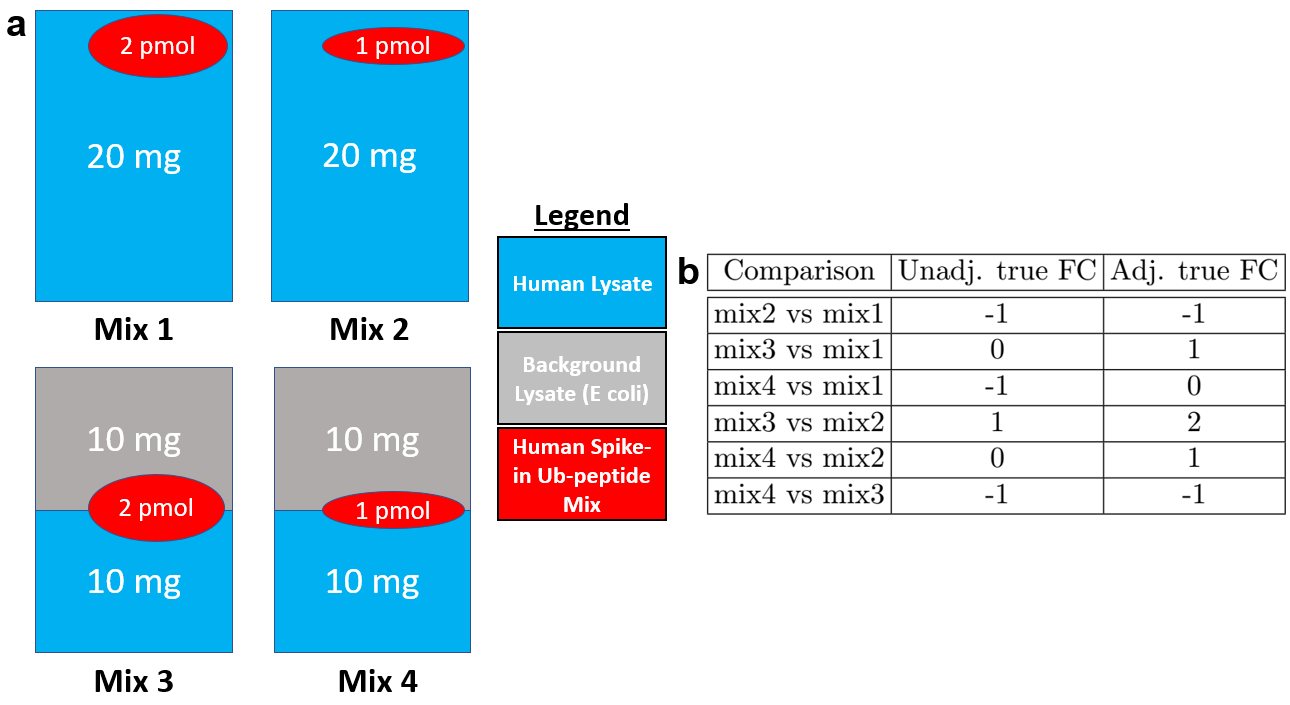
\includegraphics[scale=.4]{images/benchmark_fig.png}
\caption{{\bf Dataset 3: SpikeIn benchmark - Ubiquitination - Label-free}. (a) Relative amounts of human lysate, background {\it E. Coli} lysate, and spike-in peptides. \todo{Clarify what is changing how} (b) The expected fold change of the spike-in peptides, after adjusting for changes in the unmodified peptide (human lysate). The expected fold change is calculated using the values of the spike-in and human lysate in part (a).\todo{Could you make the columns in the table more complete? True fold-fold changes between the backgrounds; unadjusted true fold changes, adjusted true fold changes - essentially any value for any comparison that we may want to evaluate}}

\label{fig:benchmark-design}
\end{figure}

\begin{figure}[ht]
\centering
\includegraphics[scale=.6]{images/fig3.png}
\caption{
\todo{In 2a, it may be more meaningful to replace 'run' with 'bio rep'} Goals of PTM characterization, input to statistical analyses, and notation. (a) Schematic data representation, in a simplified case of two conditions and two biological replicates. Each PTM site is modeled and characterized separately, where a PTM is quantified with observed spectral features (boxes), distinguished by different charge states of a peptide. The feature \todo{log-}intensities of the PTM in Condition 1 are denoted by $y_1^\ast$ \todo{In the figure $y^*$ has 3 subscripts. Could you edit here as well?}. \todo{Log-intensities of } features corresponding to unmodified peptides in Condition 1 are denoted by $y_1$ \todo{In the figure $y$ has 3 subscripts. Could you edit here as well?}. Peptides can be fully cleaved (solid lines) and/or partially cleaved (dashed lines). \todo{OV: I am wondering whether we need Fig 2(b). The null hypothesis is specified in the text. I am not sure it is referenced anywhere. Maybe remove it for simplicity?} (b) PTM relative quantification of the population parameters by statistical inference, which makes use of the feature intensities to infer the underlying PTM abundance and protein abundance with an estimate of associated uncertainty. (c) Model-based testing for differential PTM abundance, which corrects for the underlying protein abundance with a cost of increased uncertainty about the estimate of difference between conditions.}
\label{fig:data-structure}
\end{figure}


\begin{figure}[ht]
\centering
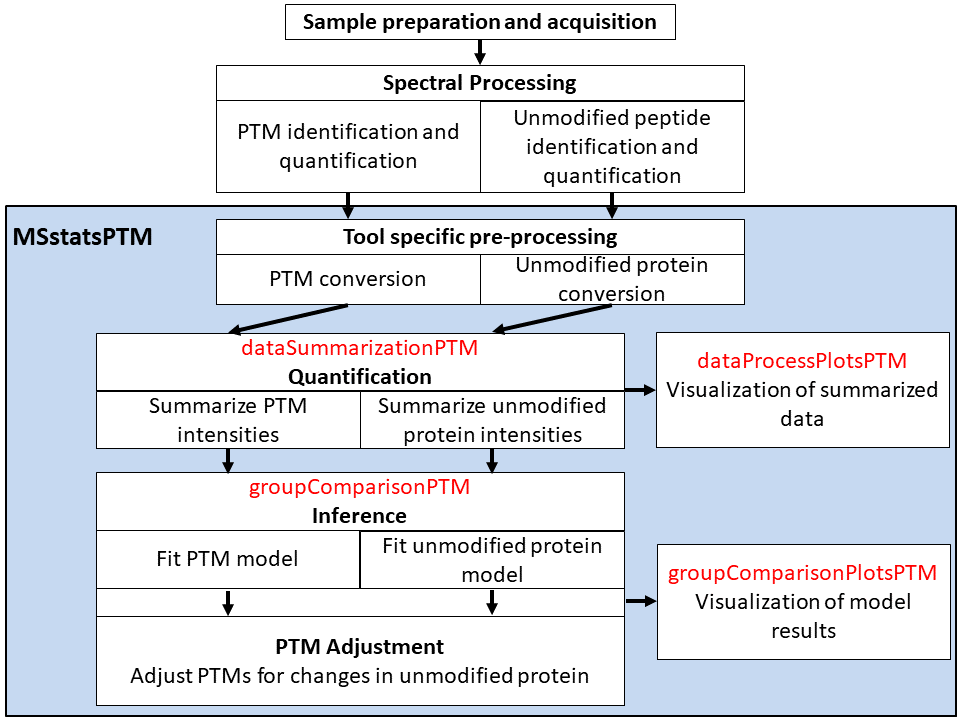
\includegraphics[scale=.8]{images/MSstatsPTM_design.png}
\caption{The workflow of $MSstatsPTM$ and how it fits into the experimental pipeline. The name of the R functions used for each step are highlighted in red. The package's workflow starts after modified and unmodified peptide quantification. First tool specific pre-processing is performed, this includes modification site identification, general data cleaning, and formatting the data into the format needed for the package. The next step is feature level summarization, which summarizes features up to the modification level for the PTM data, and the protein level for the protein data. In the final step a model is fit to identify differential PTMs and unmodified proteins across conditions and the PTM model is adjusted for changes in the unmodified protein. After both the summarization and group comparison steps, plots can be created to summarize the results.}
\label{fig:msstatsptm_design}
\end{figure}

\begin{figure}[ht]
\centering
\begin{subfigure}[c]{0.825\linewidth}
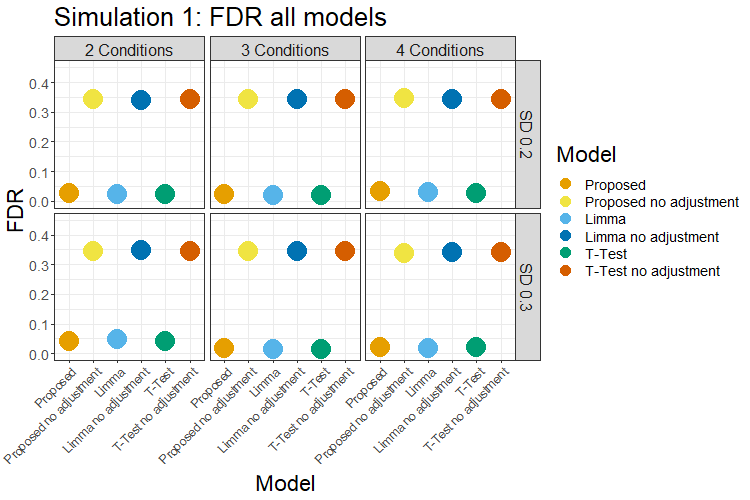
\includegraphics[width=1\textwidth]{images/sim1_FDR_all_models.png}
\caption{}
\label{fig:sim1_fdr}
\end{subfigure}
\begin{subfigure}[c]{0.825\linewidth}
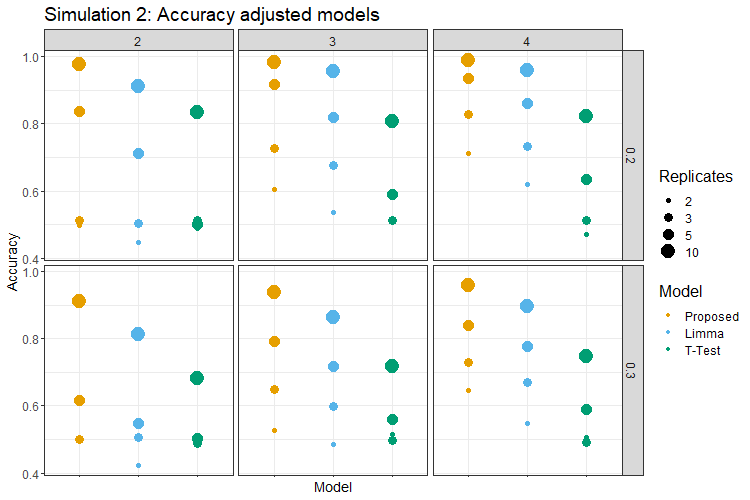
\includegraphics[width=1\textwidth]{images/sim3_Accuracy.png}
\caption{}
\label{fig:sim2_acc}
\end{subfigure}
\caption{Dataset 1 \& 2: Computer simulation. a) All the considered methods in the first computer simulation correctly calibrated FDR when adjusting for changes in protein abundance. In comparison, the methods without accounting for the protein-level changes resulted in off-target, high false positive rates. b) The advantage of using the proposed approach was apparent when including limited observations and missing values. Looking at accuracy, the proposed method outperformed Limma and $t$-test in nearly every model.
}
\label{fig:computer_sim}
\end{figure}


\begin{figure}[ht]
\centering
\begin{subfigure}[c]{0.825\linewidth}
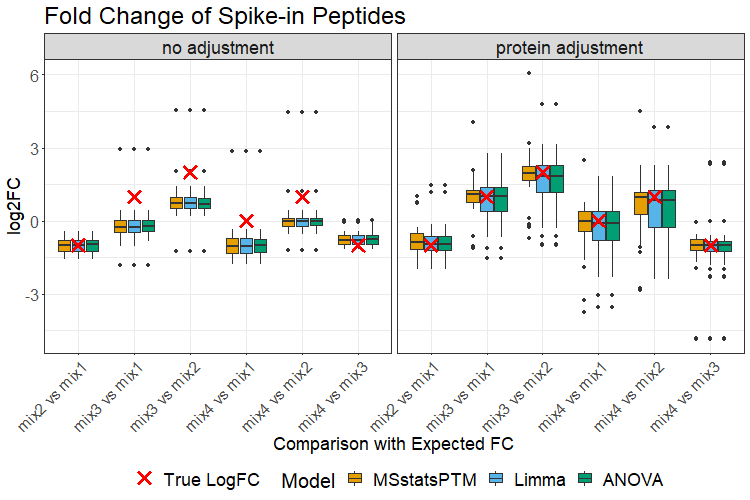
\includegraphics[width=1\textwidth]{images/spike_in_fc.png}
\caption{}
\label{fig:spikein_boxplot}
\end{subfigure}
\begin{subfigure}[c]{0.825\linewidth}
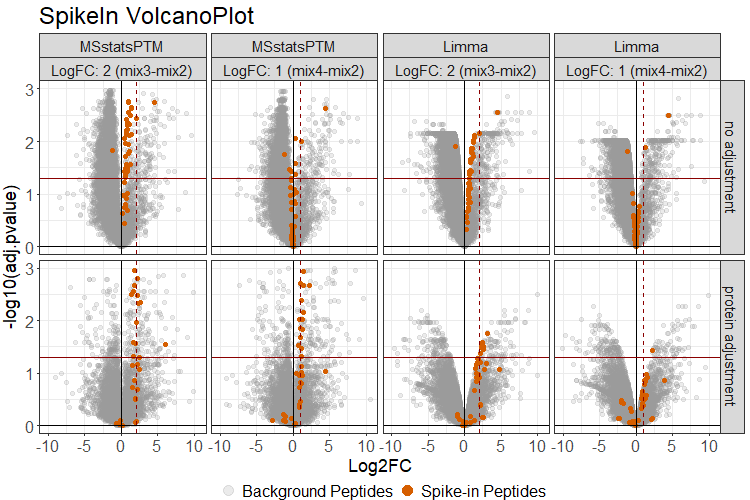
\includegraphics[width=1\textwidth]{images/spike_in_volcano.png}
\caption{}
\label{fig:spikein_prop_volcano}
\end{subfigure}
\caption{Dataset 3: SpikeIn benchmark - Ubiquitination - Label-free. a) Before adjustment the fold change of the spike-in peptides' were systematically different from the expected fold change in all models. After adjustment, this systemic difference was removed, however the inner quartile range of the Limma and $t$-test models was wider than the proposed method. b) Before adjustment the spike-in peptides (colored red) did not follow the expected log fold change; after adjustment, the spike-in peptides were more in line with expectation. Using Limma, the spike-in peptides followed the expected log fold change after adjustment, however the majority of spike-in peptides did not have a significant adjusted p-value.}
\label{fig:spikein_volcano}
\end{figure}

\begin{figure}[ht]
\centering
\begin{subfigure}[c]{0.5\linewidth}
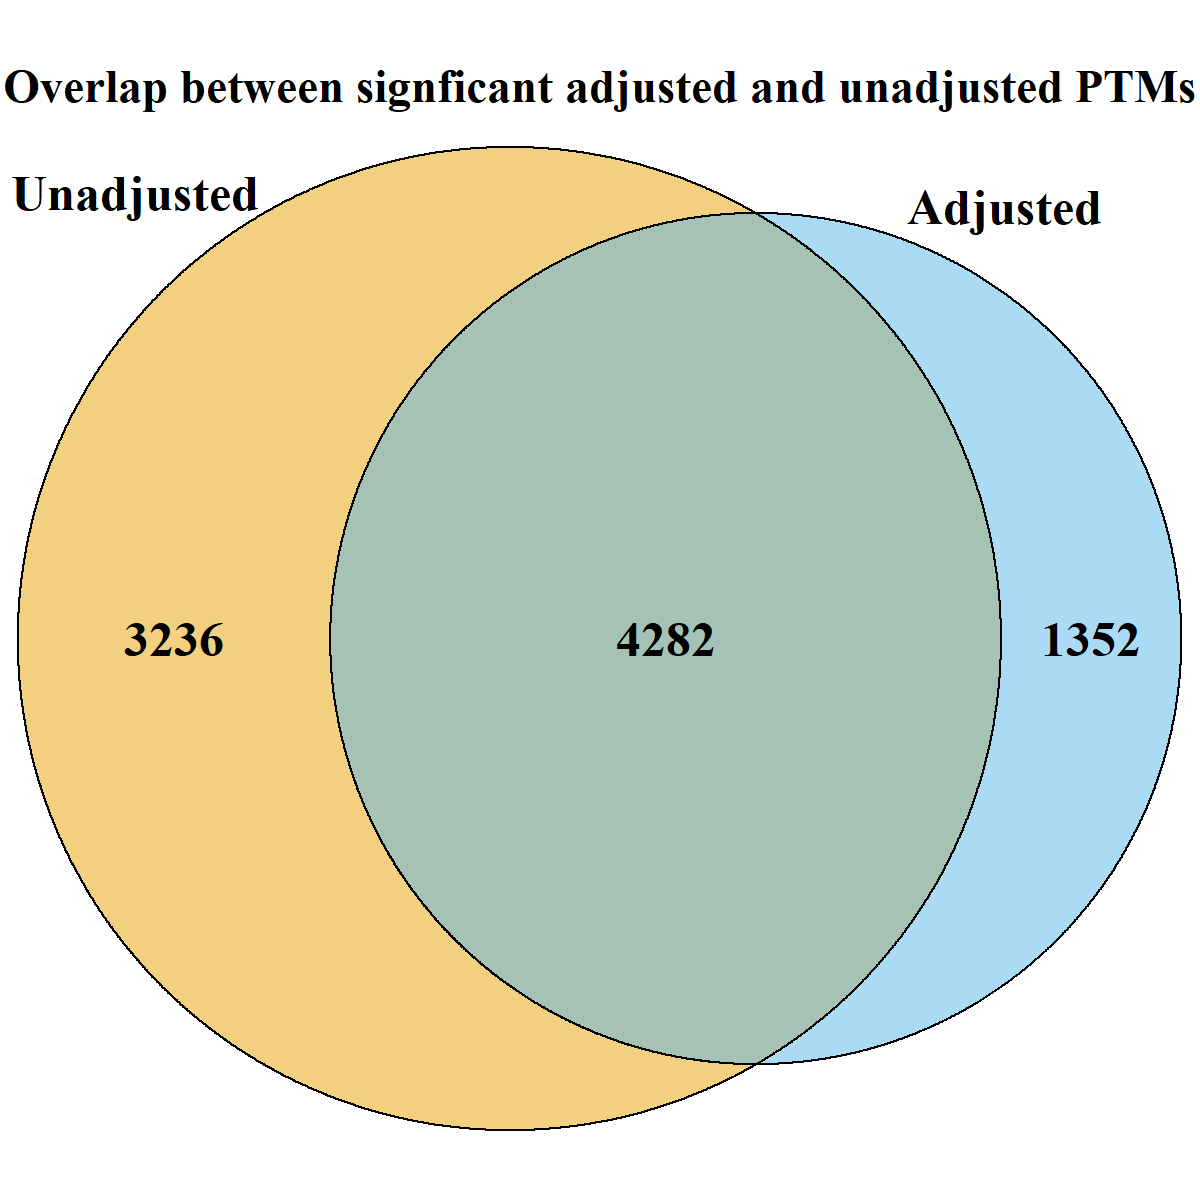
\includegraphics[width=1\textwidth]{images/ipah_venn_diagramm.png}
\caption{}
\label{fig:data4_venn_diagram}
\end{subfigure}
\begin{subfigure}[c]{0.95\linewidth}
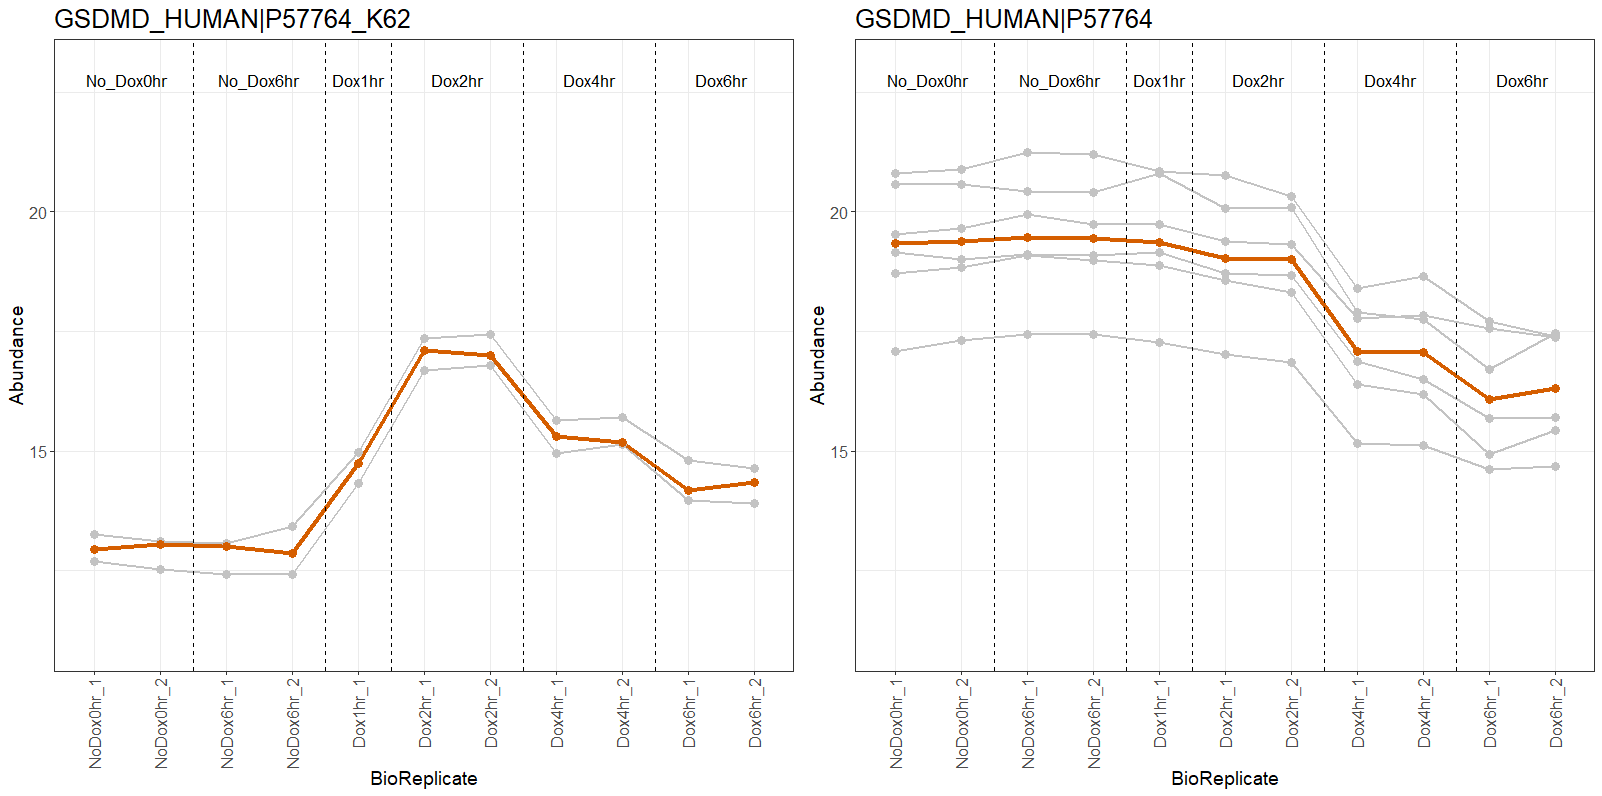
\includegraphics[width=1\textwidth]{images/IpaH_prof_plot.png}
\caption{}
\label{fig:data4_profile_plot}
\end{subfigure}
\caption{Dataset 4: Human - Ubiquitination - 1mix-TMT. a) The overlap of differential modified peptides for the PTM model with and without global protein level adjustment across all comparisons. More PTMs became insignificant after adjustment than became significant. For the peptides that became insignificant in the adjusted model, their change in abundance was driven by changes in the global protein. In contrast, peptides that became significant after adjustment had their true abundance change masked by underlying changes in the unmodified protein. b) Comparing the global profiling of protein $GSDMD$ with the ubiquitination of the protein at site $K62$. When looking at the summary of the modification and global protein it was clear the conditions follow different trends. Specifically, there appeared to be no change in abundance between Dox1hr and Dox4hr in the modified plot, however there was a large negative change when looking at the unmodified plot. This indicated the modification was confounded with changes in the unmodified protein.}
\label{fig:data4_plots}
\end{figure}

\begin{figure}[h!]
\centering
\begin{subfigure}{\textwidth}
 \centering
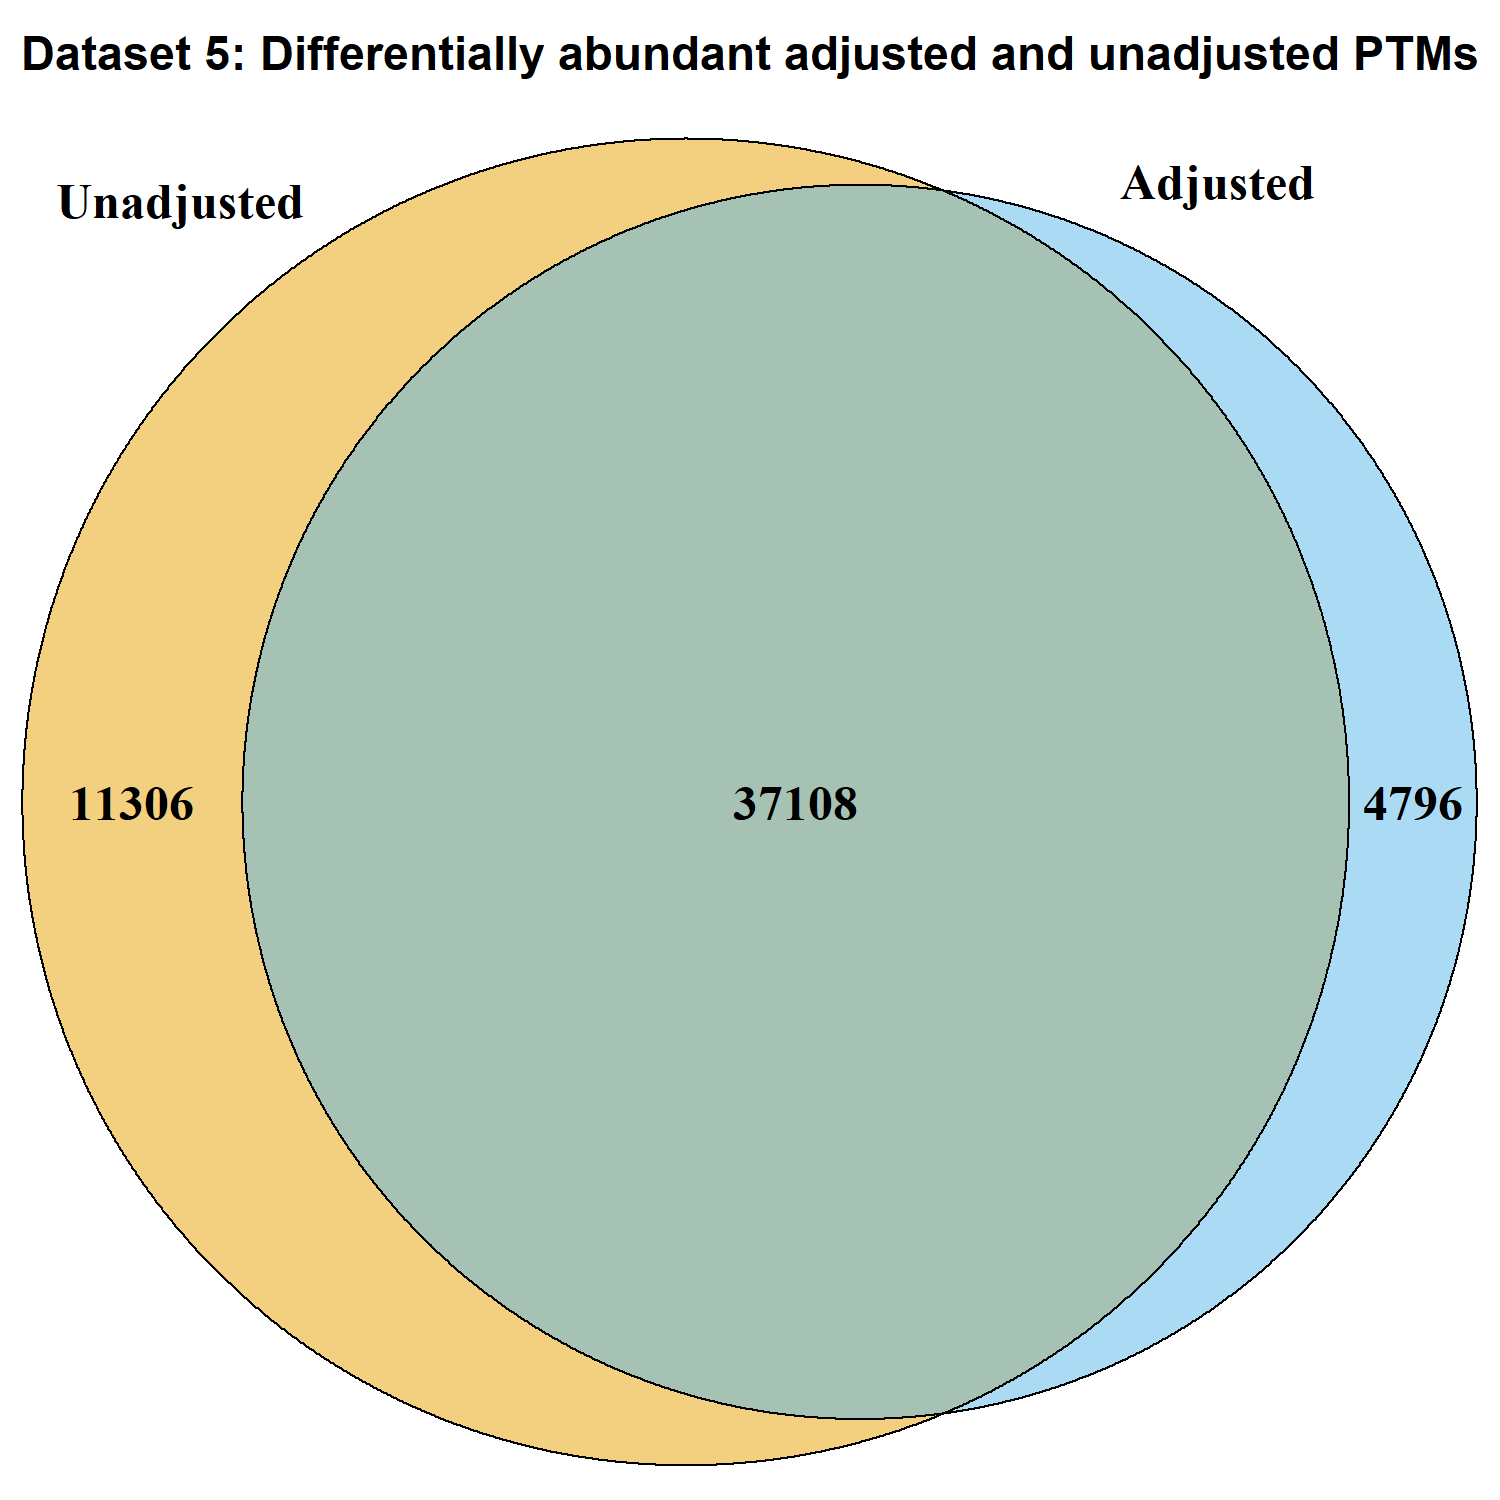
\includegraphics[height=.5\textwidth]{images/shig_venn_diagramm.png}
\caption{}
\label{fig:data5_venn_diagram}
 \end{subfigure}
 \begin{subfigure}{\textwidth}
 \centering
	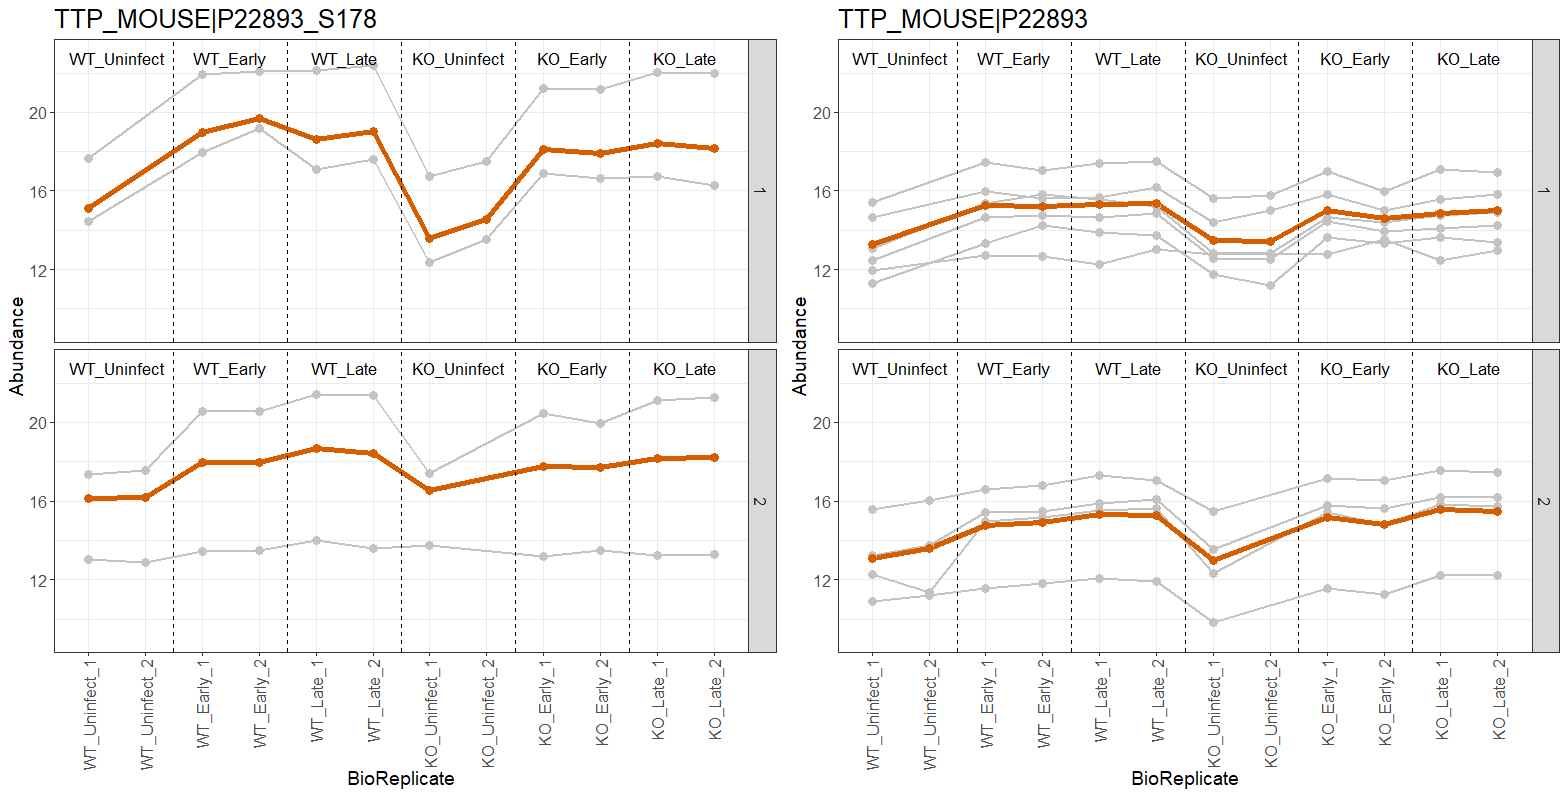
\includegraphics[width=1.0\textwidth]{images/No_Difference_Shigella_Profile_Plot}
	\caption{}
	\label{fig:data5_profile_plot}
	 \end{subfigure}
\caption{Dataset 5: Mouse - Phosphorylation - 2mix-TMT. a) The overlap of differentially modified peptides between the PTM model with and without global protein level adjustment across all comparisons. Again more PTMs became insignificant after adjustment then became significant. b) Comparing the global profiling of protein $TTP$ with the modification of the protein at site $S178$. When looking at the summary of the modification and global protein it was clear the difference between conditions followed the same trend. Specifically, there was a positive adjustment in abundance when comparing WT\_Uninfect to WT\_Late in both the modification and global profiling run. This indicated the movement was driven by changes in global protein that was only accounted for in the model after adjusting for global protein abundance change.}
\label{fig:data5_plots}
\end{figure}

\begin{figure}[h!]
\centering
 \begin{subfigure}{\textwidth}
 \centering
	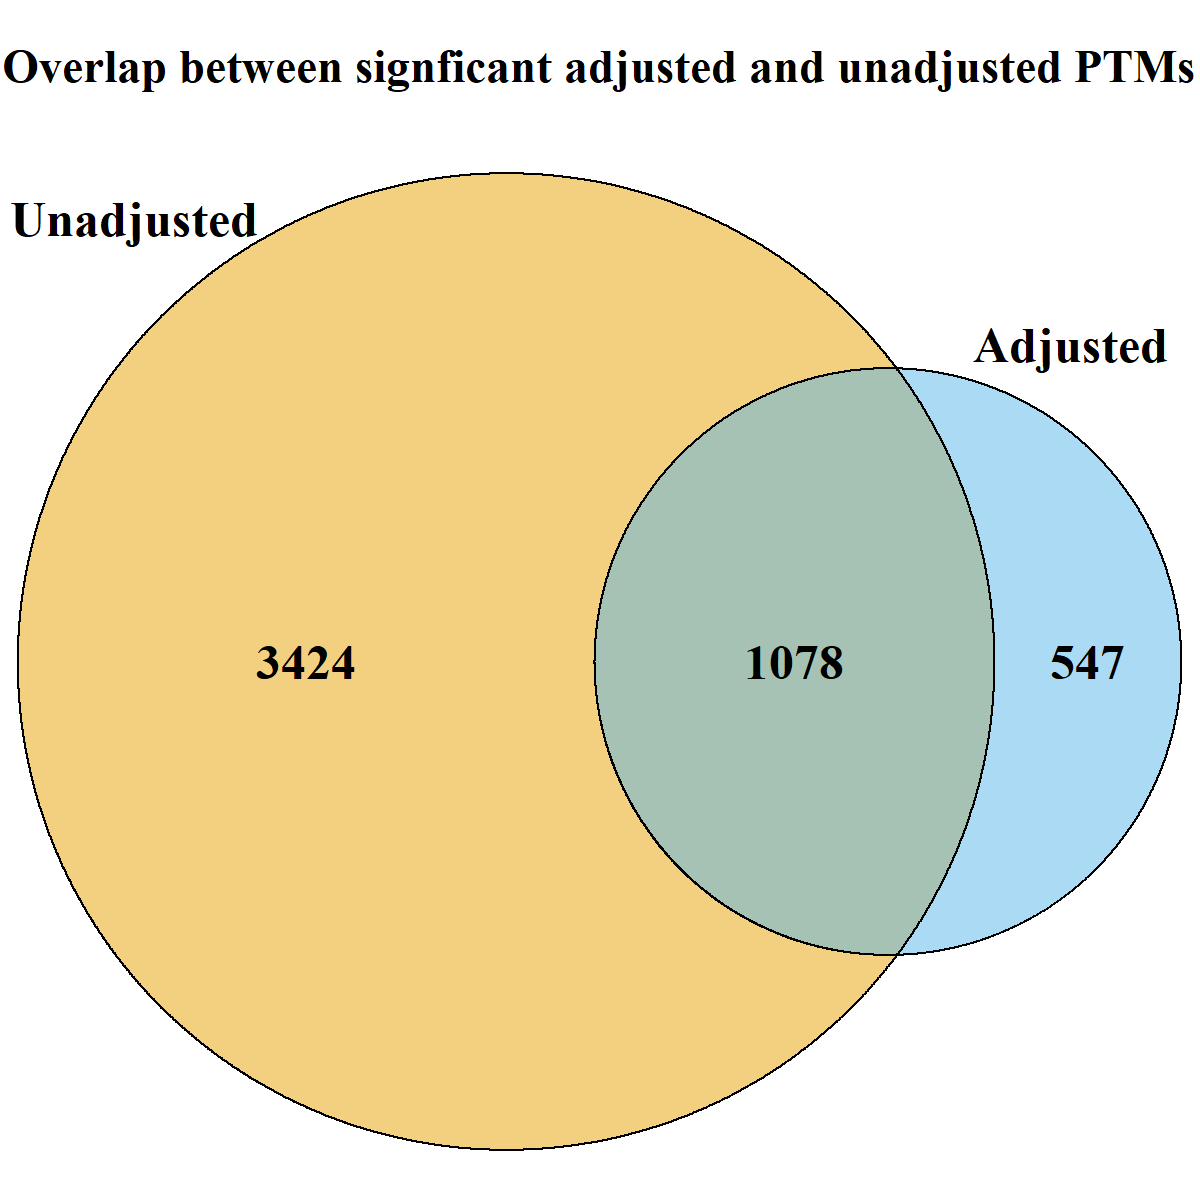
\includegraphics[height=.525\textwidth]{images/usp30_venn_diagramm}
	\caption{}
	\label{fig:data6_vd1}
 \end{subfigure}
 \begin{subfigure}{\textwidth}
 \centering
	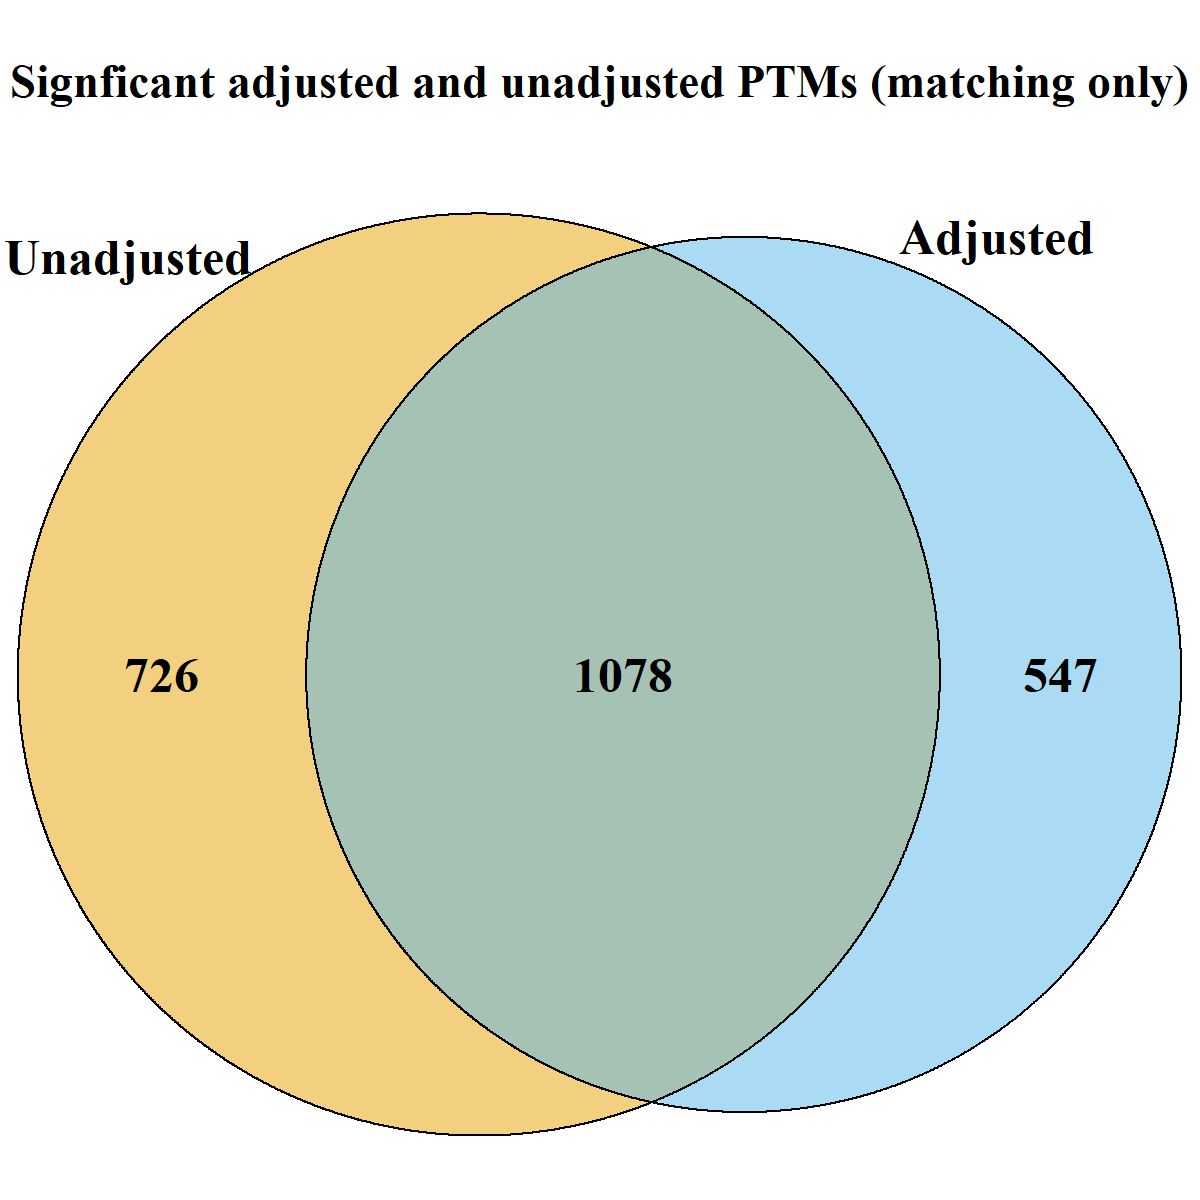
\includegraphics[height=.525\textwidth]{images/usp30_venn_diagramm_matching_only}
	\caption{}
	\label{fig:data6_vd2}
 \end{subfigure}
 \caption{Dataset 6: Human - Ubiquitination - Label-free no global profiling run. a) The overlap of differential modified peptides for the PTM model with and without global protein level adjustment across all comparisons. More PTMs became insignificant than became significant after adjustment. This was due to not having a global profiling run, resulting in a lack of overlap between modified peptides and unmodified proteins. b) Here we made the same comparison but only looked at modified peptides where adjustment could be performed, ie they had a matching unmodified protein. In this case there were significantly less peptides that became insignificant after adjustment. This highlighted the need for a global profiling run.}
\label{fig:data6_plots}
\end{figure}

%\begin{figure}[h!]
%\centering
% \begin{subfigure}{\textwidth}
% \centering
%	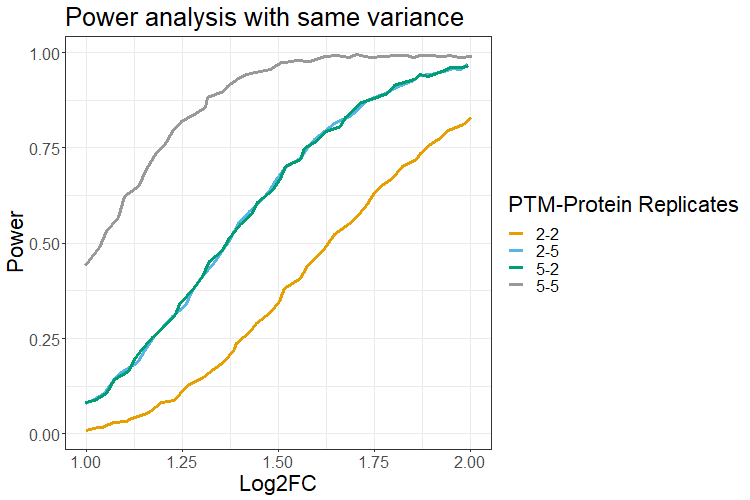
\includegraphics[width=.75\textwidth]{images/same_var_power}
%	\caption{}
% \end{subfigure}\vspace{5mm}
% \begin{subfigure}{\textwidth}
% \centering
%	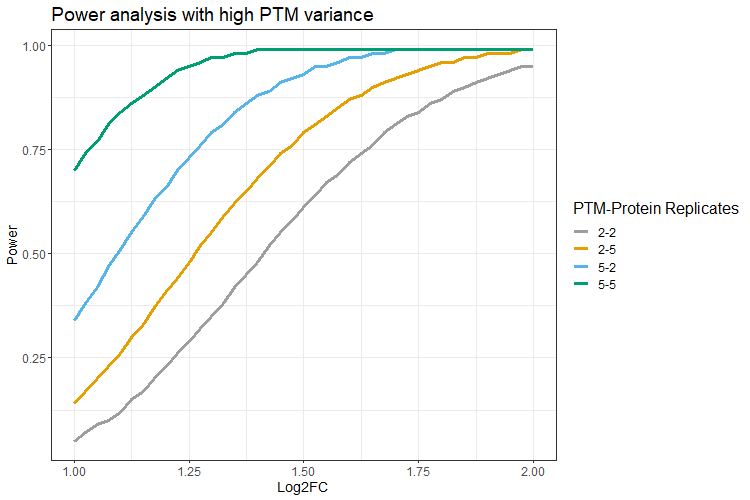
\includegraphics[width=.75\textwidth]{images/high_ptm_var_power}
%	\caption{}
% \end{subfigure}
% \caption{Power analysis of experiments with differing variances. a) The power of an experiment targeting PTMs with the same variance, .15, for the modified and unmodified peptides. Predictably when the replicates are high for both modified and unmodified peptides the power is much higher. Conversely at low replicates for each the power is much lower. The interesting part of this chart is when the replicates are different between runs. With equal variance, it does not matter if the PTM replicates or protein replicates are higher. b) In this chart the variance for the PTM is higher than the unmodified protein. The PTM variance is .2, while the unmodified protein variance is .1. With equal replicates the results are the same as above, more replicates equals more power. When the replicates are not the same we can clearly see that having more replicates for the PTM leads to higher power.}
%\label{fig:power_sd_combo}
%\end{figure}


\end{document}
